\documentclass[10pt]{article}

\usepackage{fontspec}
\usepackage[fontset=none,scheme=plain]{ctex}
\setCJKmainfont[AutoFakeBold=2,AutoFakeSlant=.2]{Songti SC}
\setCJKsansfont{Heiti SC}
\setCJKmonofont{Songti SC}
\usepackage{url}
\usepackage{booktabs}
\usepackage{amsfonts}
\usepackage{amsmath}
\usepackage{amssymb}
\usepackage{xcolor}
\usepackage{graphicx}
\usepackage{multirow}
\usepackage{enumitem}
\usepackage{array}
\usepackage{natbib}
\usepackage[top=0.86in,bottom=0.86in,left=0.9in,right=0.9in]{geometry}
\usepackage{upquote}
\usepackage{hyperref}
\usepackage{float}
\usepackage{microtype}

\hypersetup{
  colorlinks=true,
  linkcolor=blue!45!black,
  citecolor=green!35!black,
  urlcolor=blue!55!black
}
\setlist{nosep,leftmargin=2em}
\setlength{\parindent}{2em}
\setlength{\parskip}{0.2em}
\linespread{1.08}
\renewcommand{\abstractname}{摘要}
\renewcommand{\refname}{参考文献}
\renewcommand{\figurename}{图}
\renewcommand{\tablename}{表}

\title{\textbf{办公工作后训练提升软件工程能力：\\跨领域迁移的行为学解释}}

\author{
  Logan Ritchie\thanks{通讯作者：\texttt{research@surgehq.ai}}，
  Sushant Mehta，Liudas Panavas，Edwin Chen\\
  Surge AI
}

\date{}

\begin{document}

\maketitle

\begin{abstract}
长时程任务要求智能体在嵌套且存在分支的工作过程中维持连贯的状态与目标。我们将这种能力称为\emph{目标导向执行}（goal-directed execution，GDE）：它反复运用四类行为，即选择目标、构建与任务相关的状态、忠实维持更高层目标，以及对照环境验证任务是否完成。我们假设，长时程后训练能够跨领域强化这些行为。为检验这一假设，我们使用来自办公工作流的 363 个长时程多工具智能体（Long-Horizon Multi-Tool Agent，LHMTA）任务，对 Qwen3.5-122B-A10B 进行后训练。该任务集合不包含任何软件工程任务，但模型在 SWE-Bench Pro 上的 pass@1 仍提高了 5.8 个百分点。匹配轨迹分析表明，在办公工作流和软件代码仓库中，GDE 的四类行为均有所改善。SWE-Bench Pro 的汇总统计也显示，信息收集、实现和验证行为发生了相应变化。综合来看，这些结果支持一种行为学解释：长时程后训练改变了模型在任务中组织和运用知识的方式，其影响超出了训练领域。
\end{abstract}

\section{引言}
\label{sec:intro}

人们通常依据训练样例的内容与领域来描述后训练。然而，长时程任务也可能锻炼更广泛的行为组织方式。在一项复杂任务中，智能体必须决定下一步要实现什么，保持对环境的准确认识，在局部工作期间维持更高层要求，并判断自己的行动是否成功。即便工具和主题发生变化，这些要求仍会反复出现。

我们使用\emph{目标导向执行}（GDE）描述智能体持续沿正确方向推进的能力：在嵌套且存在分支的工作过程中维持连贯的目标和任务相关状态，并利用二者随时间选择、协调和评估行为。我们通过四项行为能力对 GDE 进行操作化定义：

\begin{enumerate}
  \item \textbf{目标形成：}根据父目标和当前工作状态推导出正确的即时目标。
  \item \textbf{状态构建：}收集、解释、整合并保留指导局部和更高层决策所需的环境信息。
  \item \textbf{目标稳定性：}在推进低层工作时维持更高层要求和预期结果。
  \item \textbf{验证：}判断什么证据能够证明预期状态已经达成，并在中间边界和最终边界取得这些证据。
\end{enumerate}

我们用目标循环表示任务执行。在任意层级，智能体都会形成一个目标，对环境采取行动或发起查询，根据结果更新其工作状态，再依据目标检查该状态。过于抽象而无法直接执行的行动可以分解为更低层目标，因此复杂任务包含嵌套且带分支的目标循环。GDE 正是执行这些循环，并跨层级协调其目标与状态更新所需的能力。

我们假设，GDE 是复杂智能体任务中的一种领域通用要求。因此，在一个领域中强化这种能力的训练，也可能提升模型在其他领域的表现。我们使用领域不匹配的源领域和目标领域来考察这一点。我们在 363 个 LHMTA 任务上对 Qwen3.5-122B-A10B 进行后训练；这些任务是覆盖文档、电子表格、网页研究、规划、文件操作和办公服务的真实工作流，并通过模型上下文协议工具以强化学习环境的形式提供 \citep{anthropic2024mcp}。该集合不包含软件工程任务。尽管如此，训练后的模型在 SWE-Bench Pro 上仍提高了 5.8 个百分点 \citep{deng2025swebenchpro}。

训练任务没有提供代码仓库约定、解析器语义或代码级解决方案。为了考察发生了什么变化，我们比较了相互匹配的基础模型轨迹和训练后模型轨迹。训练后的模型能够更可靠地形成服务于整体任务的局部目标，构建并维持相关工作状态，在低层工作中保留父目标要求，并验证实质性的完成条件。同样的差异既出现在办公工作流中，也出现在软件代码仓库中。

SWE-Bench Pro 的汇总统计提供了范围更广但属于间接证据的结果。在检索总量相近的情况下，训练后模型较少重复已经读取的内容；其补丁与参考实现重合得更多，同时新增行数显著更少；运行正式测试的轨迹占比则接近翻倍。目标稳定性没有干净的汇总代理指标，因此相关证据来自匹配轨迹的对比。

本文有三项贡献。第一，我们记录了从非软件领域的长时程后训练到 SWE-Bench Pro 的跨领域迁移。第二，我们通过递归目标循环表示和四项行为能力，对学习型智能体中的 GDE 进行了操作化定义。第三，我们提供了配对轨迹证据和汇总行为指标，它们与这些能力在后训练后得到提升的判断一致。GDE 为观察到的迁移提供了一种解释性说明，但所提出的、长时程任务结构与迁移之间的因果联系仍然只是一项假设。

\section{相关工作}
\label{sec:related}

\paragraph{智能体架构。}
语言智能体研究主要关注如何构建智能体：ReAct 将推理与行动交错起来 \citep{yao2023react}，Reflexion 加入语言形式的自我反思 \citep{shinn2023reflexion}，搜索方法在模型外部包装推理时探索过程 \citep{yao2023tot, zhou2024lats}，而基于分解的提示则把问题化为更简单的子问题 \citep{zhou2022least, prasad2024adapt}。近期的长时程脚手架把分解与上下文管理更直接地联系起来。HiAgent 将工作记忆组织为基于子目标的片段，以摘要替代已完成的分支，同时允许检索其细节 \citep{hu2025hiagent}。ReCAP 递归分解计划，并在子任务执行后重新引入父计划，使新的观察能够更新更高层工作 \citep{zhang2025recap}。两者都规定了改善推理时行为的结构；我们则借用相关概念描述通过后训练学得的行为。这一模式早于语言模型：分层强化学习将子任务层次作为可学习结构构建进智能体 \citep{sutton1999options, dietterich2000maxq}，HTN 规划则通过人工编写的方法分解任务 \citep{ghallab2004automated}。认知架构为完整模型提供了最接近的先例：经典的 Soar 在僵局阻塞进展时，会基于表示当前情境的工作记忆自动生成子目标 \citep{laird1987soar}；较新的 CoALA 把相同概念带入语言智能体，以工作记忆中枢组织智能体，并区分内部行动和外部行动 \citep{sumers2024coala}。所有这些贡献都在回答一个工程问题：什么机制或脚手架能让智能体表现得更好？与此同时，更广泛的趋势是追求随算力扩展、而非依赖任务特定结构的通用方法 \citep{sutton2019bitter}。我们认为，对任务完成过程的结构化解释对于理解和评估仍有价值：无论模型内部是否存在类似目标栈的结构，学习型智能体仍必须形成目标、构建状态并验证结果，因此经典术语仍适合描述智能体行为。

\paragraph{认知基础。}
目标循环表示在功能上与 \citet{miller1960plans} 的“测试--操作--测试--退出”（test-operate-test-exit，TOTE）框架一致。两者都把行为描述为递归、分层的循环：比较预期条件和所表示的当前状态，采取操作缩小差异，然后再次测试。工作状态类似于该框架中的\emph{意象}（Image），即关于有机体及其环境的、经过积累与组织的知识。该文对计划与意象更广泛的论述还包括计划形成、工作记忆、计划之间的协调，以及通过行动更新的知识。

我们通过四项行为上可观察的能力，将这一结构操作化到学习型工具使用智能体中：目标形成、状态构建、目标稳定性和验证。目标、行动、工作状态与验证是从推理、工具调用、环境反馈、编辑和测试中推断得到的，而不被视为字面意义上的内部架构。这样，该结构便可用于审计真实智能体轨迹在何处发生分歧，以及比较后训练前后的行为。其分解结构也呼应了问题空间 \citep{newell1972human}、GOMS \citep{card1983psychology} 和分层任务分析 \citep{annett1967task}。BDI 架构同样显式表示了信念状态和意图稳定性 \citep{bratman1987intention, rao1995bdi}。认知控制研究则强调在干扰下主动维持目标 \citep{miller2001integrative, duncan2012goalneglect}。

\paragraph{智能体失败的行为分析。}
我们的方法完全依据行为结构刻画智能体，沿袭了 \citet{rahwan2019machine} 提出的机器行为研究、把 GPT-3 作为认知心理学实验参与者的做法 \citep{binz2023cogpsych}，以及机器心理学的观点；后者以分析输入--输出关系而非内部机制来定义自身 \citep{hagendorff2024machine}。我们将这一范式从单轮探测扩展到长时程轨迹。越来越多的研究开始归纳智能体失败：重复循环 \citep{yao2023react}、多轮环境中的性能退化与无法恢复 \citep{laban2025lost}、规划缺陷 \citep{valmeekam2023planbench, kambhampati2024llmmodulo}，以及目标错误泛化，即智能体保有能力却追求了错误目标 \citep{langosco2022goal, shah2022goal}。目标漂移也已得到行为层面的测量，其方法包括让智能体面对相互竞争的目标，或要求智能体从临时目标返回原始目标 \citep{arike2025goaldrift}。这类工作研究提示中明确指定的顶层目标能否保持稳定；我们的解释还考虑必须在嵌套工作中保持稳定的更高层要求。每种失败模式通常只在单一任务家族中命名和测量，因此很难判断不同领域中名称不同的两种失败是否属于同一种故障。我们团队此前的工作通过分析前沿模型在真实强化学习环境中的失败，提出了智能体能力层级 \citep{ritchie2026hierarchy}；本文则把一般性的智能体失败描述为嵌套目标循环任务表示中特定位置的故障。

\paragraph{什么使训练数据具有价值。}
数据选择研究表明，数据价值并不随规模直接增长：小型精选数据集可以达到或超过完整语料库的效果 \citep{zhou2023lima, xia2024less, liu2024deita}；泛化能力随不同任务的数量和多样性而增长，而非随每个任务的样例数增长 \citep{wei2021flan, chung2022scaling, zhang2024instruction}；这一规律在程序化多样的强化学习环境中同样成立 \citep{cobbe2020procgen}。在智能体强化学习中，与现实性更高或表面相似度更高的领域相比，观察更丰富且策略轨迹更长的训练领域也与更强的跨领域能力保持相关 \citep{liu2026generalizationtax}。该分析覆盖四个环境，并且只对观察丰富度进行了干预，因此规划复杂度的作用仍是相关性的。我们团队的两项结果也指向相同方向：在大约一千份专家编写的约束评分规则上训练一个小模型，提高了它在从未见过的基准上的指令遵循能力 \citep{surge2026complexif}；在高保真企业环境 CoreCraft 上训练另一个基础模型，则提高了其在分布外工具使用基准上的表现 \citep{mehta2026corecraft}。我们的分析把这一问题扩展到跨领域迁移：第~\ref{sec:taskdesign} 节识别出一些结构性要求，它们可能有助于解释为什么在一个领域学到的行为到了另一个领域仍然有用。

\section{长时程智能体中的目标导向执行}
\label{sec:taskmodel}

我们用目标循环表示任务执行，用 GDE 描述可靠运行并协调这些循环所需的能力。这是一个行为模型：它描述智能体表面上追求什么、采取什么行动、能够获得什么证据，以及后续行为如何响应。它不假设模型内部存在字面意义上的符号目标栈或状态寄存器。

一个目标循环包含三个基本要素：

\begin{itemize}
  \item \textbf{目标：}环境的期望状态，其中也包括智能体对环境的认知。
  \item \textbf{行动：}旨在使环境向该状态转变的一次交互。
  \item \textbf{工作状态：}智能体当前对环境的表示；该表示是从行为中推断出来的，并与其活跃目标和父目标相关。
\end{itemize}

环境状态是实际为真的情况；工作状态则是智能体当前对它的表示。这里的环境足够宽泛，也包含智能体所知道的内容，因此一次调查的目标可以是弄清哪些文件相关。在最高层，目标由任务提示形成；在任务内部，局部目标是根据父目标和当前工作状态形成的即时期望状态。

智能体将工作状态与目标进行比较，选择一项行动，观察结果并更新工作状态（图~\ref{fig:goalloop}）。如果更新后的状态满足目标，循环便退出或把控制权交还给父循环；否则，更新后的状态会为下一次行动提供依据。由于智能体开始时几乎从不拥有完整知识，行动既可以改变环境，也可以揭示环境信息。打开文件、查询服务、运行测试和检查电子表格，都会更新智能体对实际情况的认识。一个行动也可以是抽象的行动序列，需要进一步分解为低层目标。

\begin{figure}[H]
\centering
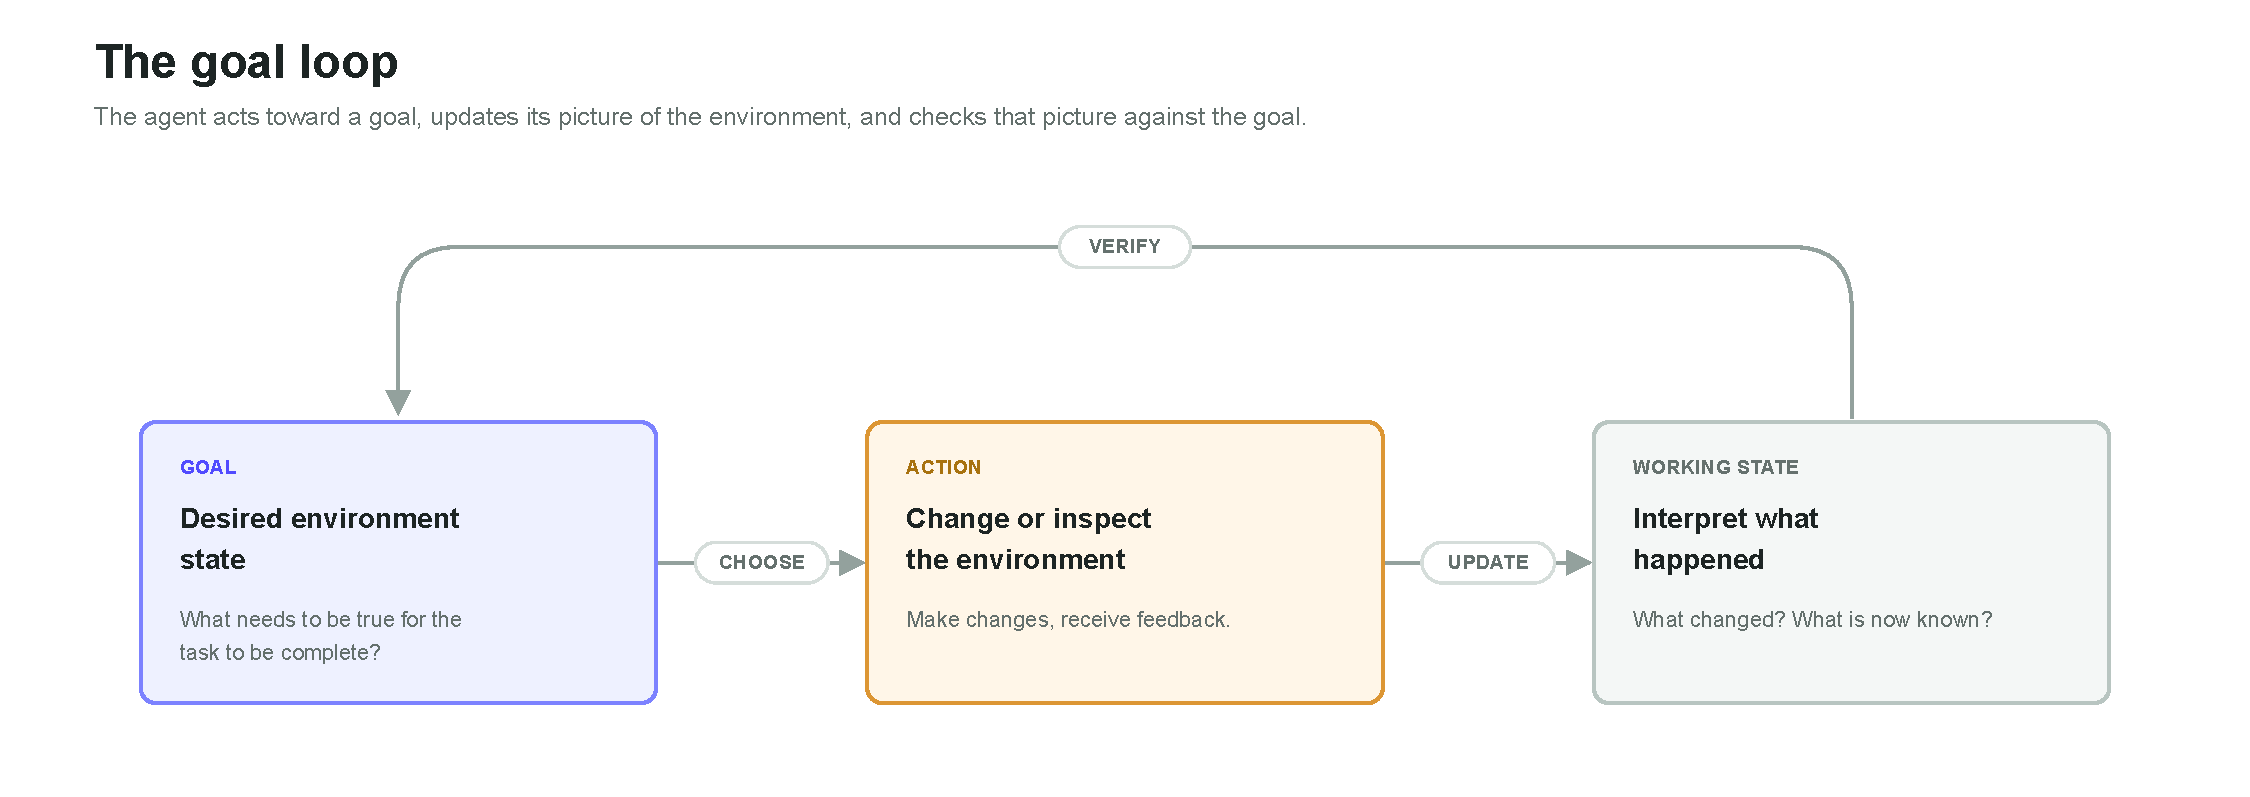
\includegraphics[width=0.75\linewidth]{figures/figure_02_goal_loop.pdf}
\caption{目标循环。智能体形成目标，对环境采取行动或发起查询，根据结果更新工作状态，再将更新后的状态与目标比较；验证把工作状态重新连接到目标。}
\label{fig:goalloop}
\end{figure}

复杂任务包含这些循环构成的层次结构。例如，审查一家公司的软件订阅，并建议哪些供应商合同应续签、重新谈判或取消，这项任务过于抽象，无法直接执行。智能体必须先将其分解：

\begin{enumerate}
  \item 找到合同和跟踪支出的财务工作簿。
  \item 明确决策标准：预算目标、使用率阈值和取消通知期限。
  \item 提取当前有效的订阅及其续约日期。
  \item 从每个工具的管理面板获取使用数据。
  \item 对数字进行归一化，使工具之间可比，例如把月度与年度计费、按席位计费与固定价格统一起来。
  \item 将支出与使用情况匹配，并标记使用不足或功能重复的工具。
  \item 调查边缘情况，例如某个使用很少、但支撑关键集成的工具。
  \item 给出续签、重新谈判或取消的建议。
\end{enumerate}

每一步都是一个运行独立循环实例的子目标，而且大多数步骤在到达具体工具调用之前还会继续分解：获取使用数据可以拆成找到各工具的管理面板、导出活动报告、处理不提供导出功能的工具，以及把结果合并到一张可比较的表格中。一项规模不大的办公任务会扩展成深达数层、宽达数十个循环的树（图~\ref{fig:goaltree}）。一些子目标按顺序执行，另一些则形成可以并行推进、之后必须综合结果的分支。

\begin{figure}[H]
\centering
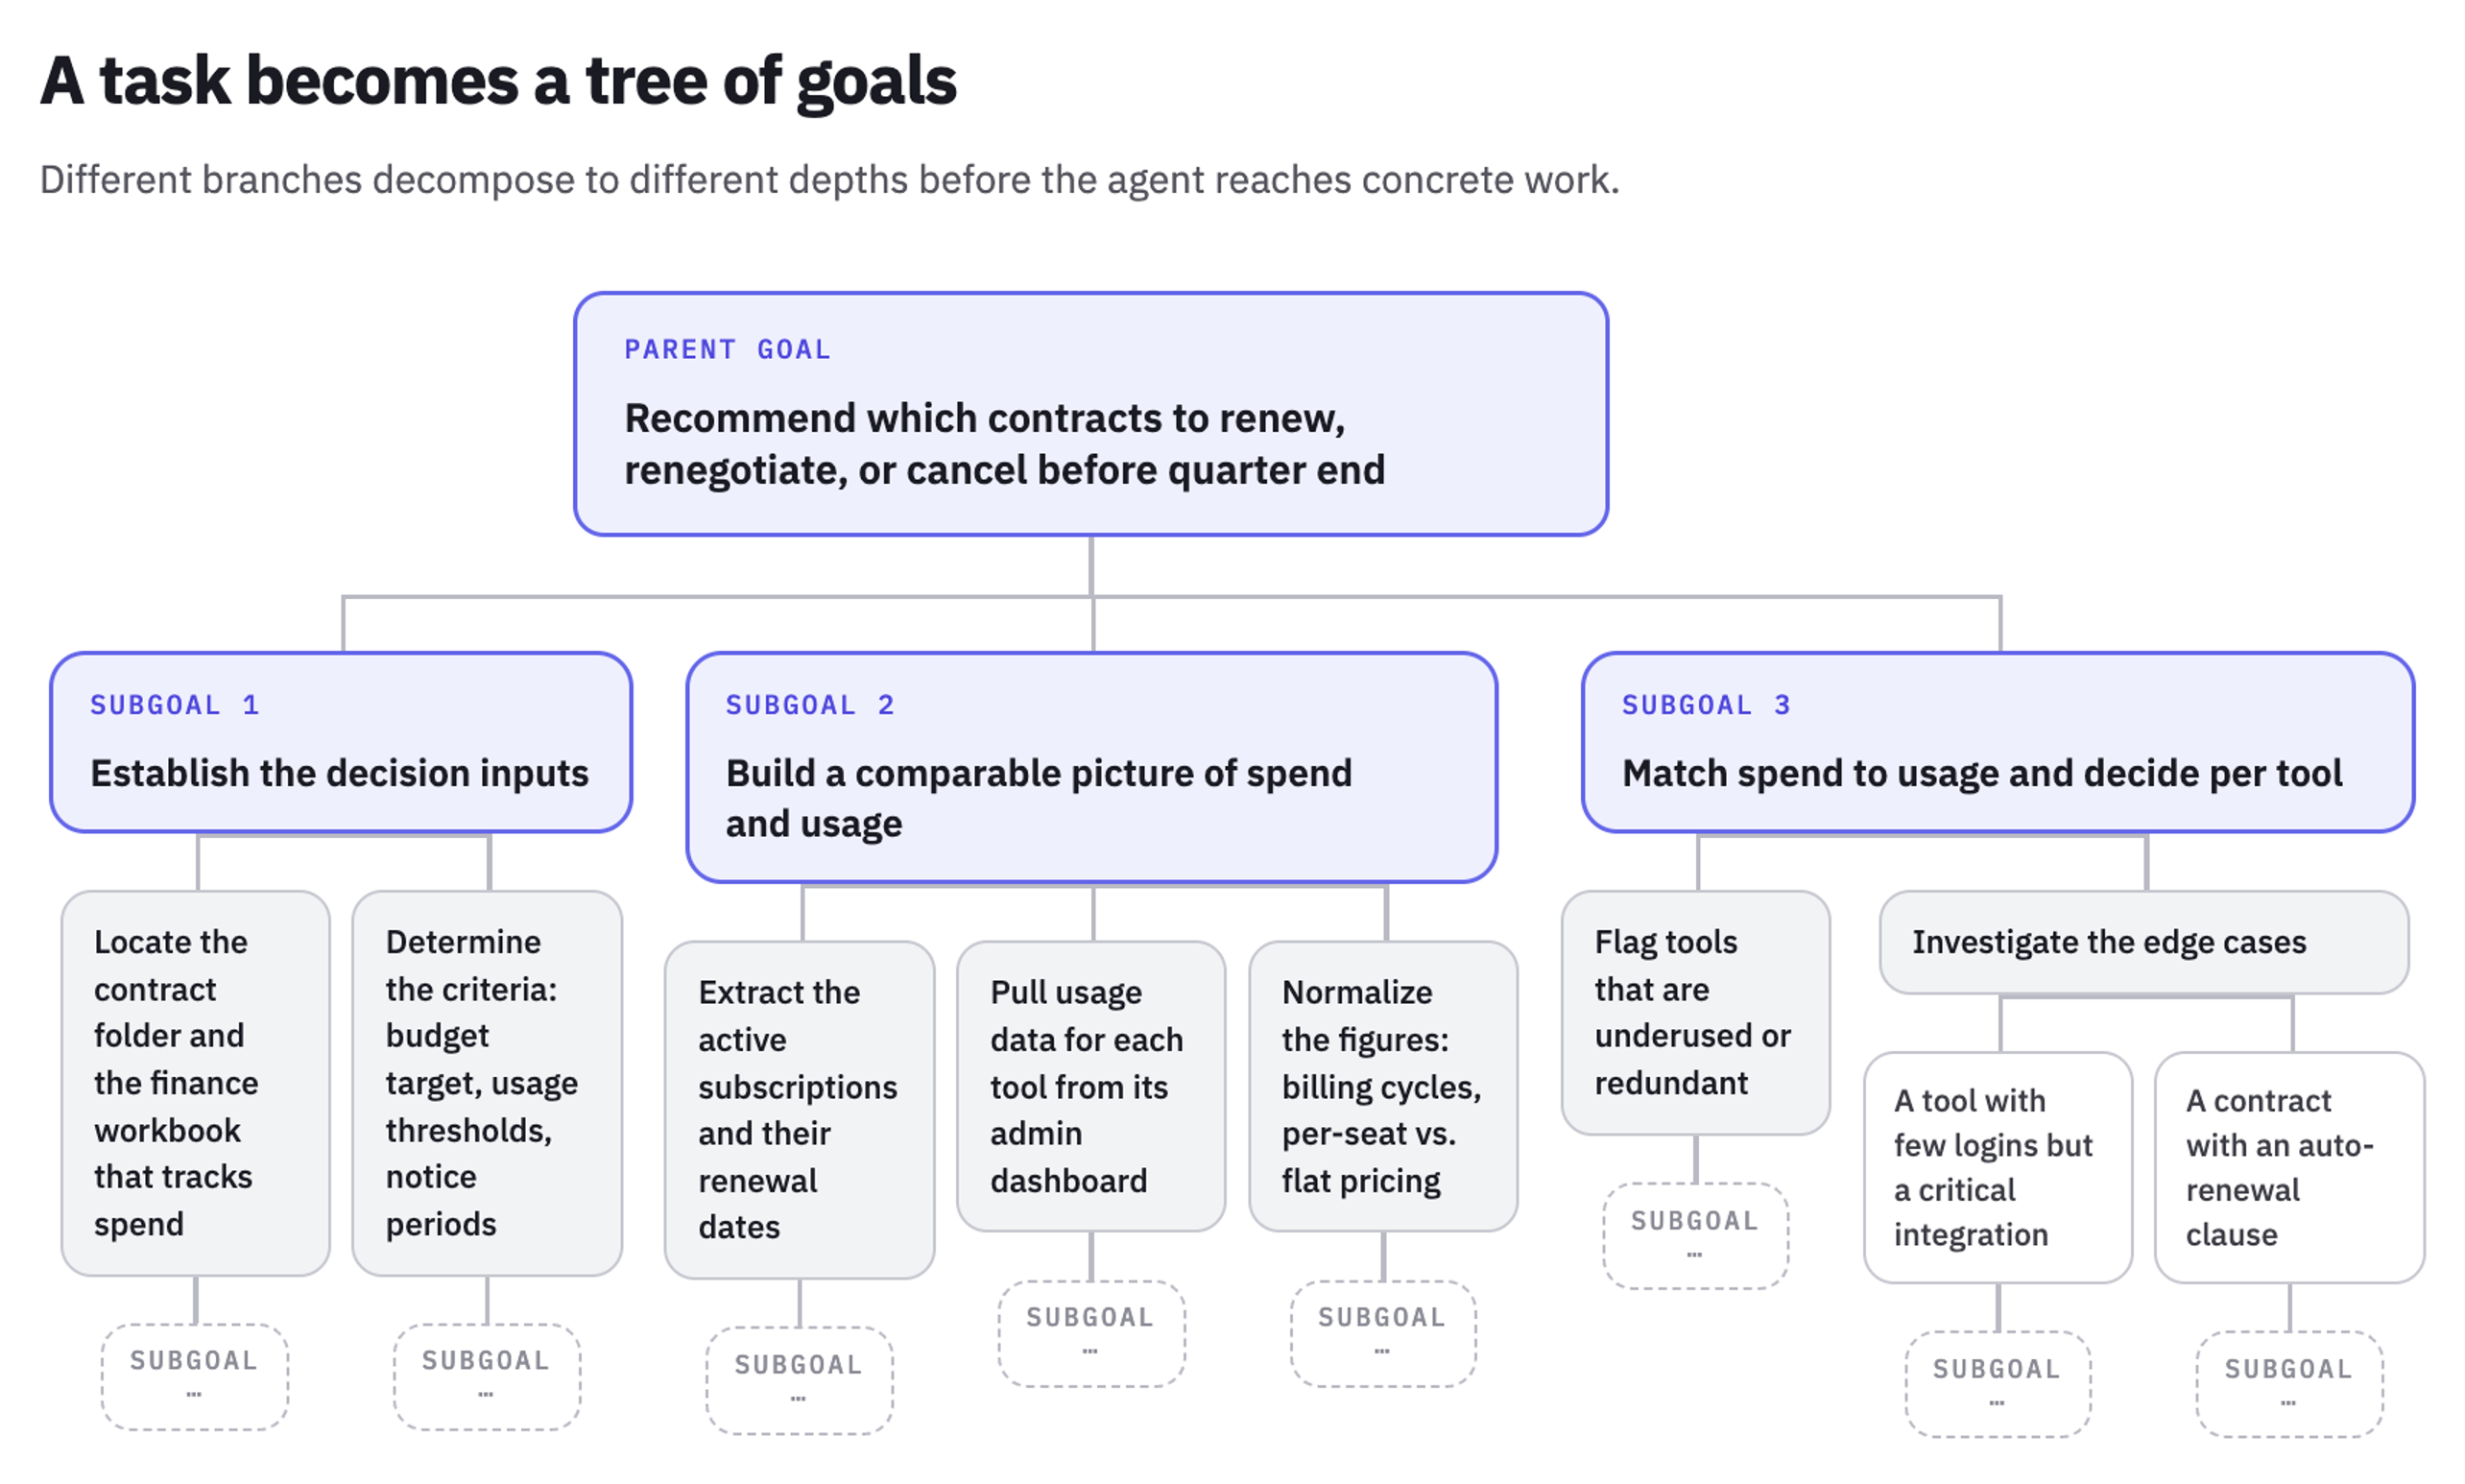
\includegraphics[width=\linewidth]{figures/tree.png}
\caption{一项任务会变成目标树。订阅审查任务被分解为带分支的子目标；在智能体到达具体工作之前，不同分支会被分解到不同深度。}
\label{fig:goaltree}
\end{figure}

分解只能解释部分困难。智能体还必须把低层观察整合进一个连贯的工作状态，并理解每项观察对当前子目标和更高层目标分别意味着什么。这种状态记录会以一些典型方式失败：

\begin{itemize}
  \item \textbf{局部合理的目标可能在全局上是错误的。}把所有合同都换算为月度成本可以简化比较，却会掩盖某份年度合同下周就自动续约这一事实，而这正是任务关注的期限。
  \item \textbf{相关事实可能在层级间丢失。}获取使用数据时，智能体注意到大部分活动由服务账户产生，但在比较时只保留了真人登录数据，结果一个使用频繁的工具看起来像是闲置的。
  \item \textbf{子任务可以成功，却破坏父目标要求。}取消一个价格低廉、很少使用的工具可以弥补预算缺口，却悄然破坏另一个保留工具所依赖的集成。
  \item \textbf{中间结果可以自洽，却并不完整。}根据财务工作簿生成的支出清单在内部是一致的，但清单本身无法暴露那些由个人银行卡报销、从未进入工作簿的订阅。
\end{itemize}

这些例子展示了我们用来操作化定义 GDE 的四项能力会如何失效（图~\ref{fig:failurepoints}）。表~\ref{tab:capabilities} 给出了每类失效的一般形式。

\begin{figure}[H]
\centering
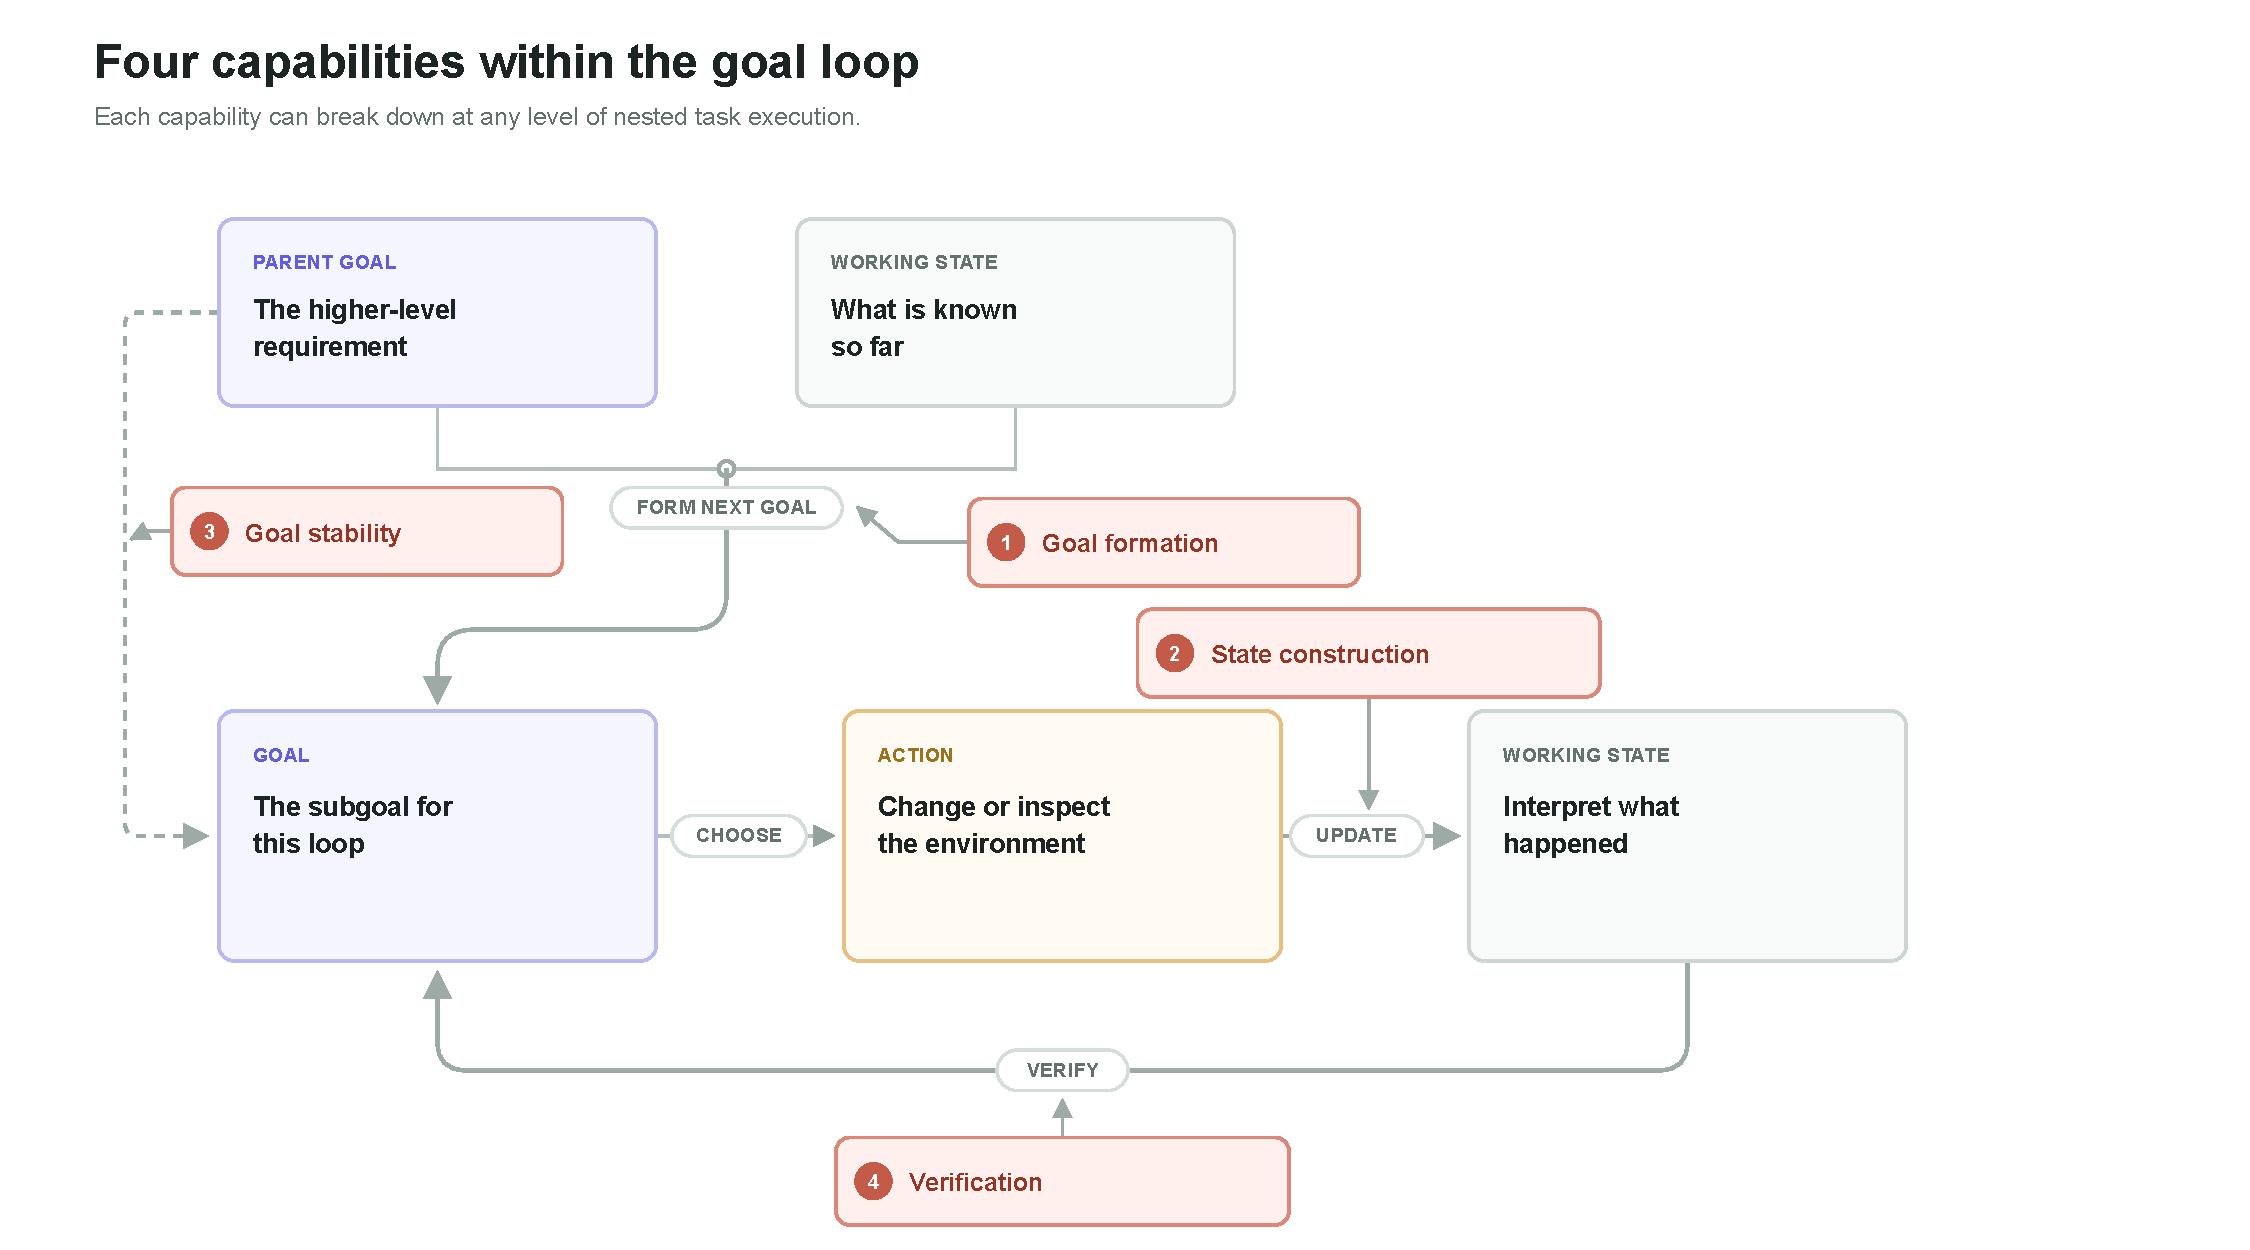
\includegraphics[width=0.85\linewidth]{figures/figure_04_failure_points.pdf}
\caption{目标循环中的四项能力：目标形成、状态构建、目标稳定性和验证。每项能力都可能在嵌套任务执行的任意层级失效。}
\label{fig:failurepoints}
\end{figure}

\begin{table}[H]
\centering
\caption{四项能力及其可能的失效方式。}
\label{tab:capabilities}
\begin{tabular}{p{0.24\linewidth}p{0.68\linewidth}}
\toprule
能力 & 失效方式 \\
\midrule
目标形成 & 模型根据父目标和工作状态得出了错误的局部目标：它可能是一个更简单的代理目标、范围错误的目标，或一个局部合理但在更广情境下错误的目标。 \\
\addlinespace
状态构建 & 模型遗漏、丢弃了理解环境与目标之间关系所需的信息，或未能把这些信息组合起来。 \\
\addlinespace
目标稳定性 & 局部障碍或复杂子目标取代了模型原本正确表示的更高层目标。 \\
\addlinespace
验证 & 模型在整体任务或中间子目标层级跳过验证，或依赖局部结果或代理指标。 \\
\bottomrule
\end{tabular}
\end{table}

目标循环在功能上与 TOTE 一致 \citep{miller1960plans}：两者都描述递归、分层的循环，将预期条件与所表示的当前状态比较，采取操作缩小差异，然后再次测试。我们使用这一结构的目的有所不同。我们从学习型工具使用智能体的行为中推断其组成要素，并使用四项能力比较不同训练条件和不同领域中的轨迹。

\section{任务结构与迁移假设}
\label{sec:taskdesign}

我们的迁移假设是，不同领域的任务可能对 GDE 提出相似要求。LHMTA 任务旨在复现真实工作的复杂性，其设计专门针对四类任务要求：

\begin{itemize}
  \item \textbf{深层分解：}高层目标需要被拆分为许多并行或顺序执行的子任务。
  \item \textbf{并行调查与综合：}决策所需证据分散在不同文件、服务和工具中。
  \item \textbf{相互纠缠的约束：}高层要求彼此交互，使局部决策变得困难。
  \item \textbf{长依赖链：}后续工作依赖早期提取、解释和修改步骤的正确性。
\end{itemize}

这些要求可能同时锻炼多项能力（图~\ref{fig:taskdifficulty}）。例如，深层分解反复要求形成目标；并行调查要求根据分散证据构建状态；相互纠缠的约束会对目标稳定性施加压力；长依赖链则使中间验证格外重要，因为一个未经检查的错误会污染之后的每一步。相关的跨领域强化学习结果发现，观察丰富度和策略轨迹长度与泛化能力相关 \citep{liu2026generalizationtax}，但并未分离本文讨论的递归结构。这些关系为迁移假设提供了动机，但本实验没有分离它们的因果效应。

\begin{figure}[H]
\centering
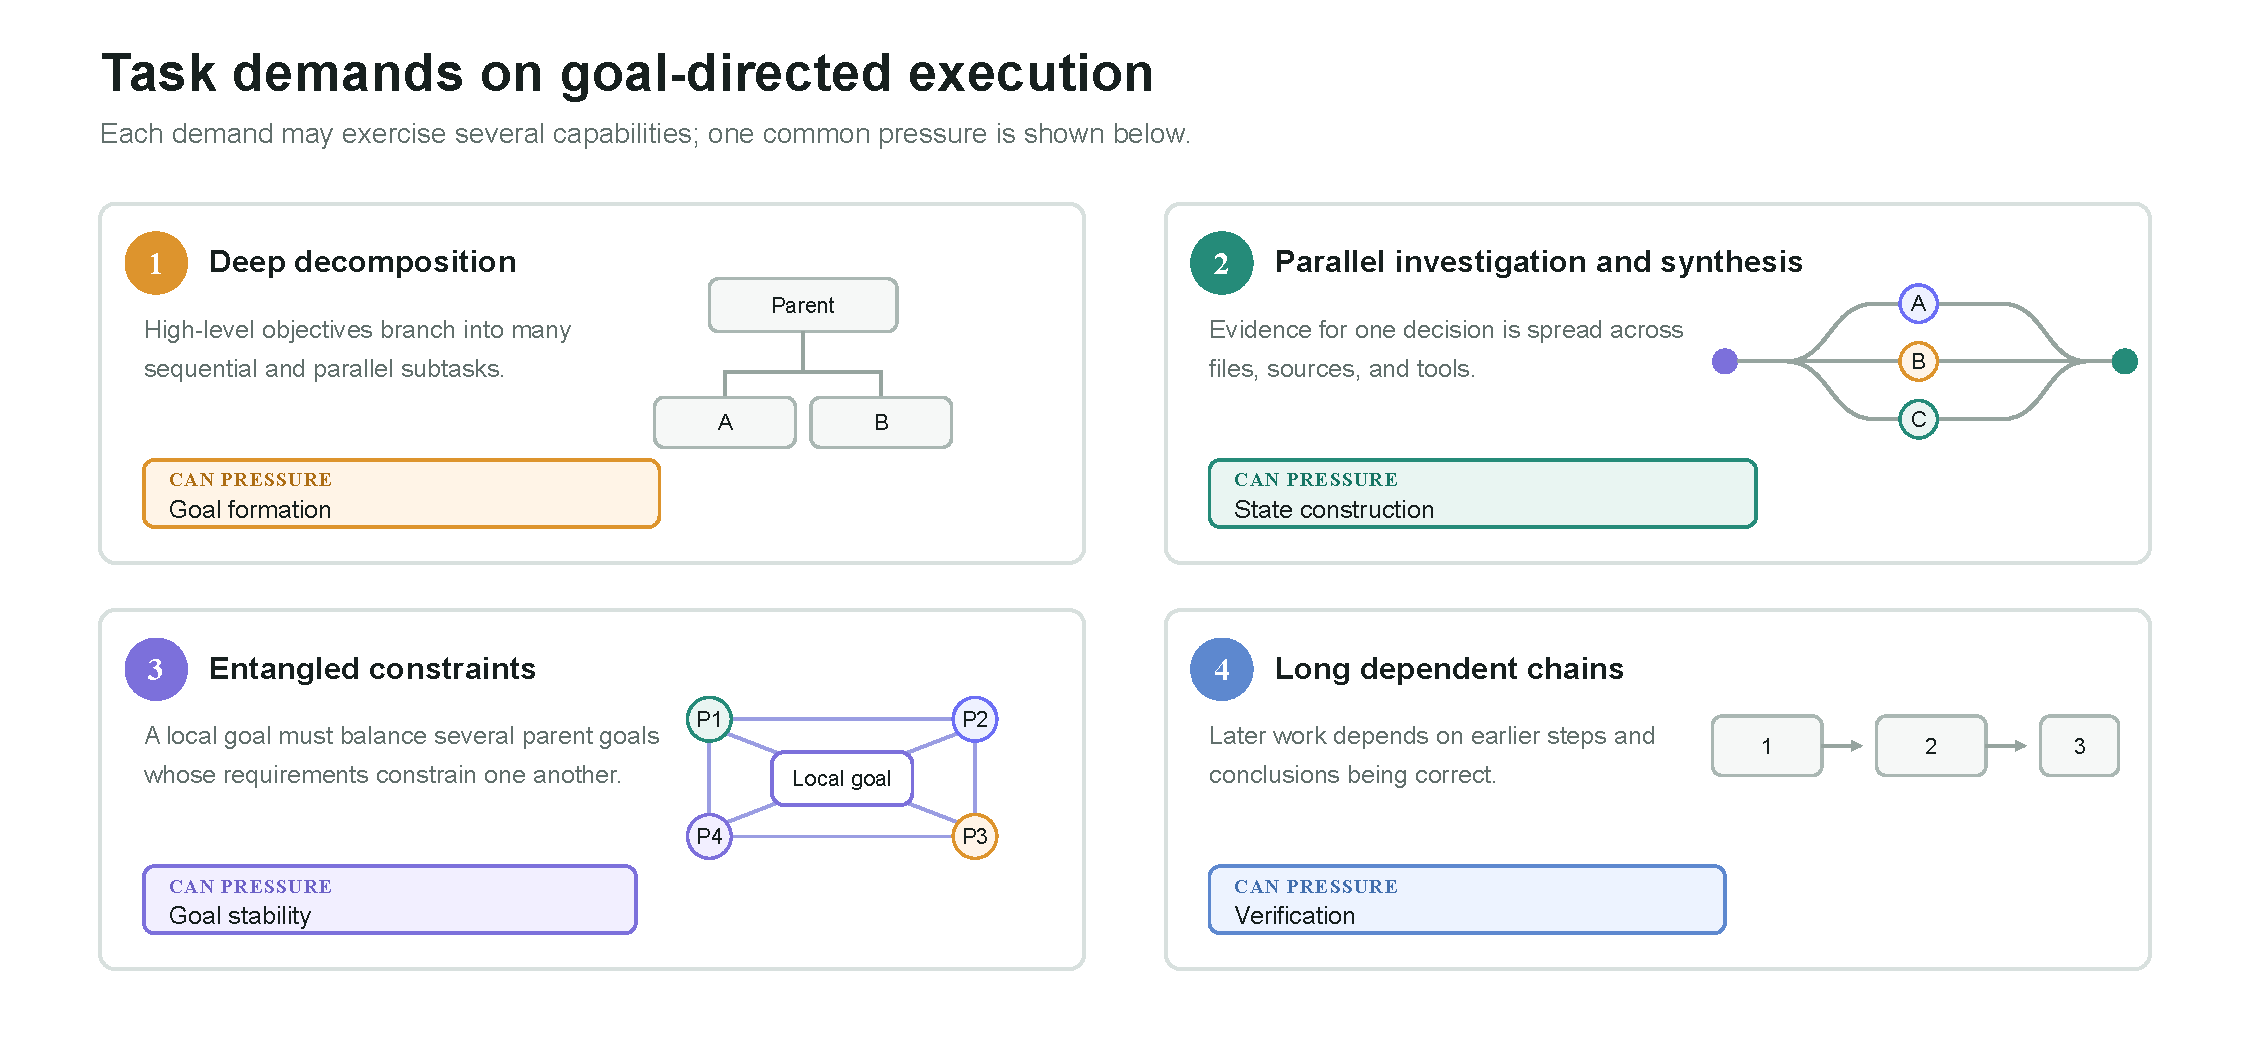
\includegraphics[width=0.85\linewidth]{figures/figure_05_task_difficulty.pdf}
\caption{LHMTA 中的四类任务要求：深层分解、并行调查与综合、相互纠缠的约束，以及长依赖链。每一类要求都可能锻炼 GDE 的多个方面；图中突出显示了每类要求常见的一种压力。}
\label{fig:taskdifficulty}
\end{figure}

工具和主题的广度使模型接触到这些要求的多样实例。与某个电子表格库、工具模式或输出模板绑定的捷径，只能对集合中的一小部分任务有用；相比之下，改进行动与目标、环境状态之间关系的能力，则可以在不同任务间持续发挥作用。

为了展示一个真实任务的规模，我们把一条成功的 LHMTA 轨迹重建为递归任务图。每个节点记录一个目标、采取的行动和得到的状态；子节点表示分解出的子任务，并行分支表示可独立推进的工作，后继节点则汇总它们的结果。一个证据目录把建模节点与相应的轨迹事件连接起来。

重建后的层次结构包含：

\begin{center}
\begin{tabular}{lr}
\toprule
结构指标 & 数值 \\
\midrule
任务级目标循环节点 & 53 \\
最大嵌套深度 & 10 个任务层级 \\
叶子子任务 & 29 \\
并行扇出点 & 3 \\
最大并行扇出宽度 & 5 个子任务 \\
顺序后继或综合节点 & 21 \\
源轨迹中的工具调用 & 42 \\
归一化轨迹事件 & 120 \\
\bottomrule
\end{tabular}
\end{center}

完整重建结果及其证据目录以\href{https://logan-surge.github.io/lhmta-task-decomposition/}{交互式任务分解}形式提供。它展示了单个任务的结构复杂度，但没有用于数据集或训练效果的汇总分析。

\section{实验设置与结果}
\label{sec:setup}

实验比较了两个领域：源领域是长时程办公与一般工具使用工作流，目标领域是软件工程。训练集合不包含软件工程任务、评分器或基准反馈。这两个领域在主题和工具上不同，但都要求管理长而有状态的任务。

\subsection{训练环境}
\label{sec:environment}

LHMTA 由通过模型上下文协议服务器提供的真实专业工作流组成。其 27 个任务类别覆盖文档、电子表格和幻灯片操作；搜索与检索；文件管理；日程与日历；浏览器自动化；规划；以及跨办公服务的工具使用。单个任务通常要求智能体在一条轨迹内协调多个服务。该集合不包含软件工程任务。

每项任务都配有一个确定性的 Python 评分器，它根据若干标准评估最终环境状态。只有满足全部标准，任务才能获得严格的通过判定；而按标准划分的结构会提供部分得分训练信号。成功轨迹通常包含 30 至 40 个工具调用轮次和 80,000 至 100,000 个词元。

任务作者以强模型无法可靠完成的真实工作为设计目标，并在整个集合层面监控工具、任务类型和失败模式的多样性。本实验使用的数据集快照包含 403 项任务：其中 363 项用于训练，40 项留作分布内评估。

\subsection{训练}
\label{sec:training}

基础模型为 Qwen3.5-122B-A10B，这是一种开放权重的混合专家模型，总参数量为 1220 亿，激活参数约为 100 亿。我们使用 LoRA 对其注意力投影和 MLP 投影进行适配 \citep{hu2022lora}。

训练分为两个阶段。首先，模型在 Kimi K2.6 针对 LHMTA 任务生成的 3,000 条轨迹上进行监督预热；这些轨迹经过拒绝采样，仅保留得分高于 0.9 的轨迹。预热使强化学习变得可行：基础策略很少能完成足够多的长时程任务内容，以至于无法获得稀疏的通过/失败奖励。

其次，我们使用 GSPO 序列级估计器在全部 363 项任务上进行训练 \citep{zheng2025gspo}。每个提示采样八条 rollout，每条完整轨迹获得的稠密奖励等于其满足的评分标准比例。奖励在轨迹层级分配，而不是分配给单独的工具调用前缀。评估采用各基准的原生评分，而不是训练时的稠密奖励。

SFT 教师只在 LHMTA 任务上生成轨迹；外部基准没有提供任何训练任务、评分器、检查点选择信号、超参数调优信号或奖励设计信号。

\subsection{评估}
\label{sec:evaluation}

我们在分布内留出集和外部基准上比较了基础检查点与训练后检查点。Toolathlon 衡量跨异构工具的长时程编排能力 \citep{li2025toolathlon}，BFCL-V4 评估函数调用 \citep{patil2025bfcl}，SWE-Bench Pro 则要求智能体解决真实代码仓库中的问题 \citep{deng2025swebenchpro}。所有结果均为贪心解码下的 pass@1。

表~\ref{tab:toolresults} 给出了分布内留出集和外部工具使用基准的结果。留出集结果证明模型在目标训练环境中有所提升；Toolathlon 与 BFCL-V4 则表明，一部分增益超出了 LHMTA 的特定任务、评分器和工具约定。

\begin{table}[H]
\centering
\small
\caption{基础检查点和训练后检查点在分布内及外部工具使用任务上的结果。}
\label{tab:toolresults}
\begin{tabular}{llrrr}
\toprule
基准 & 领域关系 & 基础模型 pass@1 & 训练后 pass@1 & 变化 \\
\midrule
LHMTA 留出集 & 分布内 & 10.0\% & 27.5\% & +17.5pp \\
Toolathlon & 外部工具使用 & 22.2\% & 31.8\% & +9.6pp \\
BFCL-V4 & 外部函数调用 & 55.7\% & 59.2\% & +3.5pp \\
\bottomrule
\end{tabular}
\end{table}

表~\ref{tab:sweresults} 给出了本文考察的跨领域结果：尽管训练集合不包含任何软件工程任务，SWE-Bench Pro 的性能仍然有所提升。仅凭基准迁移无法识别模型行为发生了什么变化。第~\ref{sec:analysis} 节考察该迁移是否与更强的 GDE 相一致。

\begin{table}[H]
\centering
\caption{相同检查点在跨领域 SWE-Bench Pro 上的性能。}
\label{tab:sweresults}
\begin{tabular}{lrrr}
\toprule
基准 & 基础模型 pass@1 & 训练后 pass@1 & 变化 \\
\midrule
SWE-Bench Pro & 20.5\% & 26.3\% & +5.8pp \\
\bottomrule
\end{tabular}
\end{table}

\section{跨领域迁移的行为分析}
\label{sec:analysis}

\subsection{方法}
\label{sec:method}

我们分析了所有基础模型失败而训练后模型成功的 103 项任务：其中包括 12 个 LHMTA 留出集案例、77 个 SWE-Bench Pro 案例和 14 个 Toolathlon 案例。每个案例都比较了同一任务上，在相同提示、环境、脚手架和评估协议下得到的基础模型轨迹与训练后模型轨迹，共计 206 条轨迹。我们选择这个按结果筛选的子集，是为了研究新近成功的行为如何表现出来。该子集不能估计每项能力在完整评估分布中的普遍程度。

我们使用 Claude Opus 4.8 作为根因分析智能体。对于每个评分输出失败，该智能体从失败轨迹向前回溯，识别轨迹偏离成功路径的、最早受到证据支持的位置。它考察任务要求、评估器证据、工具调用与结果、生成的工件、编辑、测试及模型推理。每份报告都引用支持其因果解释的具体轨迹事件与工件，使我们能够依据源材料审计报告。成功轨迹只为任务正确的路径提供对照证据，并不被自动视作真实标准。

这些报告通过定位和记录候选分歧点加速了分析；它们并未独立验证本文框架。我们依据相应的原始轨迹人工审查报告，在把任何案例用作示例之前，将其中的主张和引文与原始推理消息、工具调用、环境响应、编辑和测试逐一核对。通过在案例间反复比较，我们把反复出现的行为差异组织为四项能力：目标形成、状态构建、目标稳定性和验证。这些能力构成一个解释框架，而不是互斥标签。

我们还在相互匹配的 SWE-Bench Pro 轨迹上，以确定性指标补充案例研究。这些指标涵盖检索重复度与广度、是否接触参考补丁所改动的文件、补丁大小，以及是否运行正式测试与测试发生的时机。它们提供了范围更广、但仍属间接的行为变化信号。

\subsection{配对轨迹中的四项能力}
\label{sec:capabilities}

表~\ref{tab:manifestations} 总结了每项能力在配对示例中的表现。表层失败因领域而异，但每一对案例都体现了当前目标、更高层要求和环境证据之间相同的关系破裂。

\begin{table}[H]
\centering
\small
\caption{四项能力在一般工具使用案例和软件工程案例配对中的表现。}
\label{tab:manifestations}
\begin{tabular}{p{0.16\linewidth}p{0.38\linewidth}p{0.38\linewidth}}
\toprule
能力 & 一般工具使用中的表现 & 软件工程中的表现 \\
\midrule
目标形成 & 选择了一个局部合理、却与任务含义冲突的计算方式 & 尽管已有辅助函数编码了所需语义，仍重新实现相同行为 \\
\addlinespace
状态构建 & 丢弃父目标所需的公式计算值 & 未能把新要求与代码仓库现有的验证结构联系起来 \\
\addlinespace
目标稳定性 & 重新加入了一门违反此前识别出的课程层级约束的课程 & 为满足一个过时的局部测试而改变正确的解析器行为 \\
\addlinespace
验证 & 把有范围限制的提取结果当作完整目录 & 检查了新导出，却让下游调用方继续调用已删除的 API \\
\bottomrule
\end{tabular}
\end{table}

\paragraph{目标形成。}
每个循环都需要把提示或父行动转换为一个具体目标，该目标必须同时以更高层目标和环境为依据。常见失败模式是选择一个局部合理、却在更广情境中错误的目标。

\textbf{SWE-Bench Pro：NodeBB 的选定字段。}任务要求 NodeBB 数据库调用方从存储对象中请求选定字段。两个模型都找到了已经实现所需选定字段语义的辅助函数和测试，其中包括为每个键保留一个结果，以及把请求了但不存在的字段表示为 \texttt{null}。正确的局部目标应是让公共方法通过这些辅助函数执行。基础模型却在后端路径中重新实现字段过滤，并改变了对象不存在时的行为。训练后模型则复用了既有辅助函数，包括 Postgres 路径中的函数。

\textbf{Toolathlon：A/B 转化率。}任务要求计算首页点击转化为商店浏览的频率。基础模型尚未检查任何数值，就把转化率定义为 \texttt{clicks / store\_views}。这一计算产生超过 100\% 的比率后，模型虽然指出结果异常，却仍继续执行。训练后模型结合父目标解释各列，并使用 \texttt{store\_views / clicks}。在两个领域中，差异都在于环境信息如何塑造下一个局部目标（图~\ref{fig:goalcontrast}）。

\begin{figure}[H]
\centering
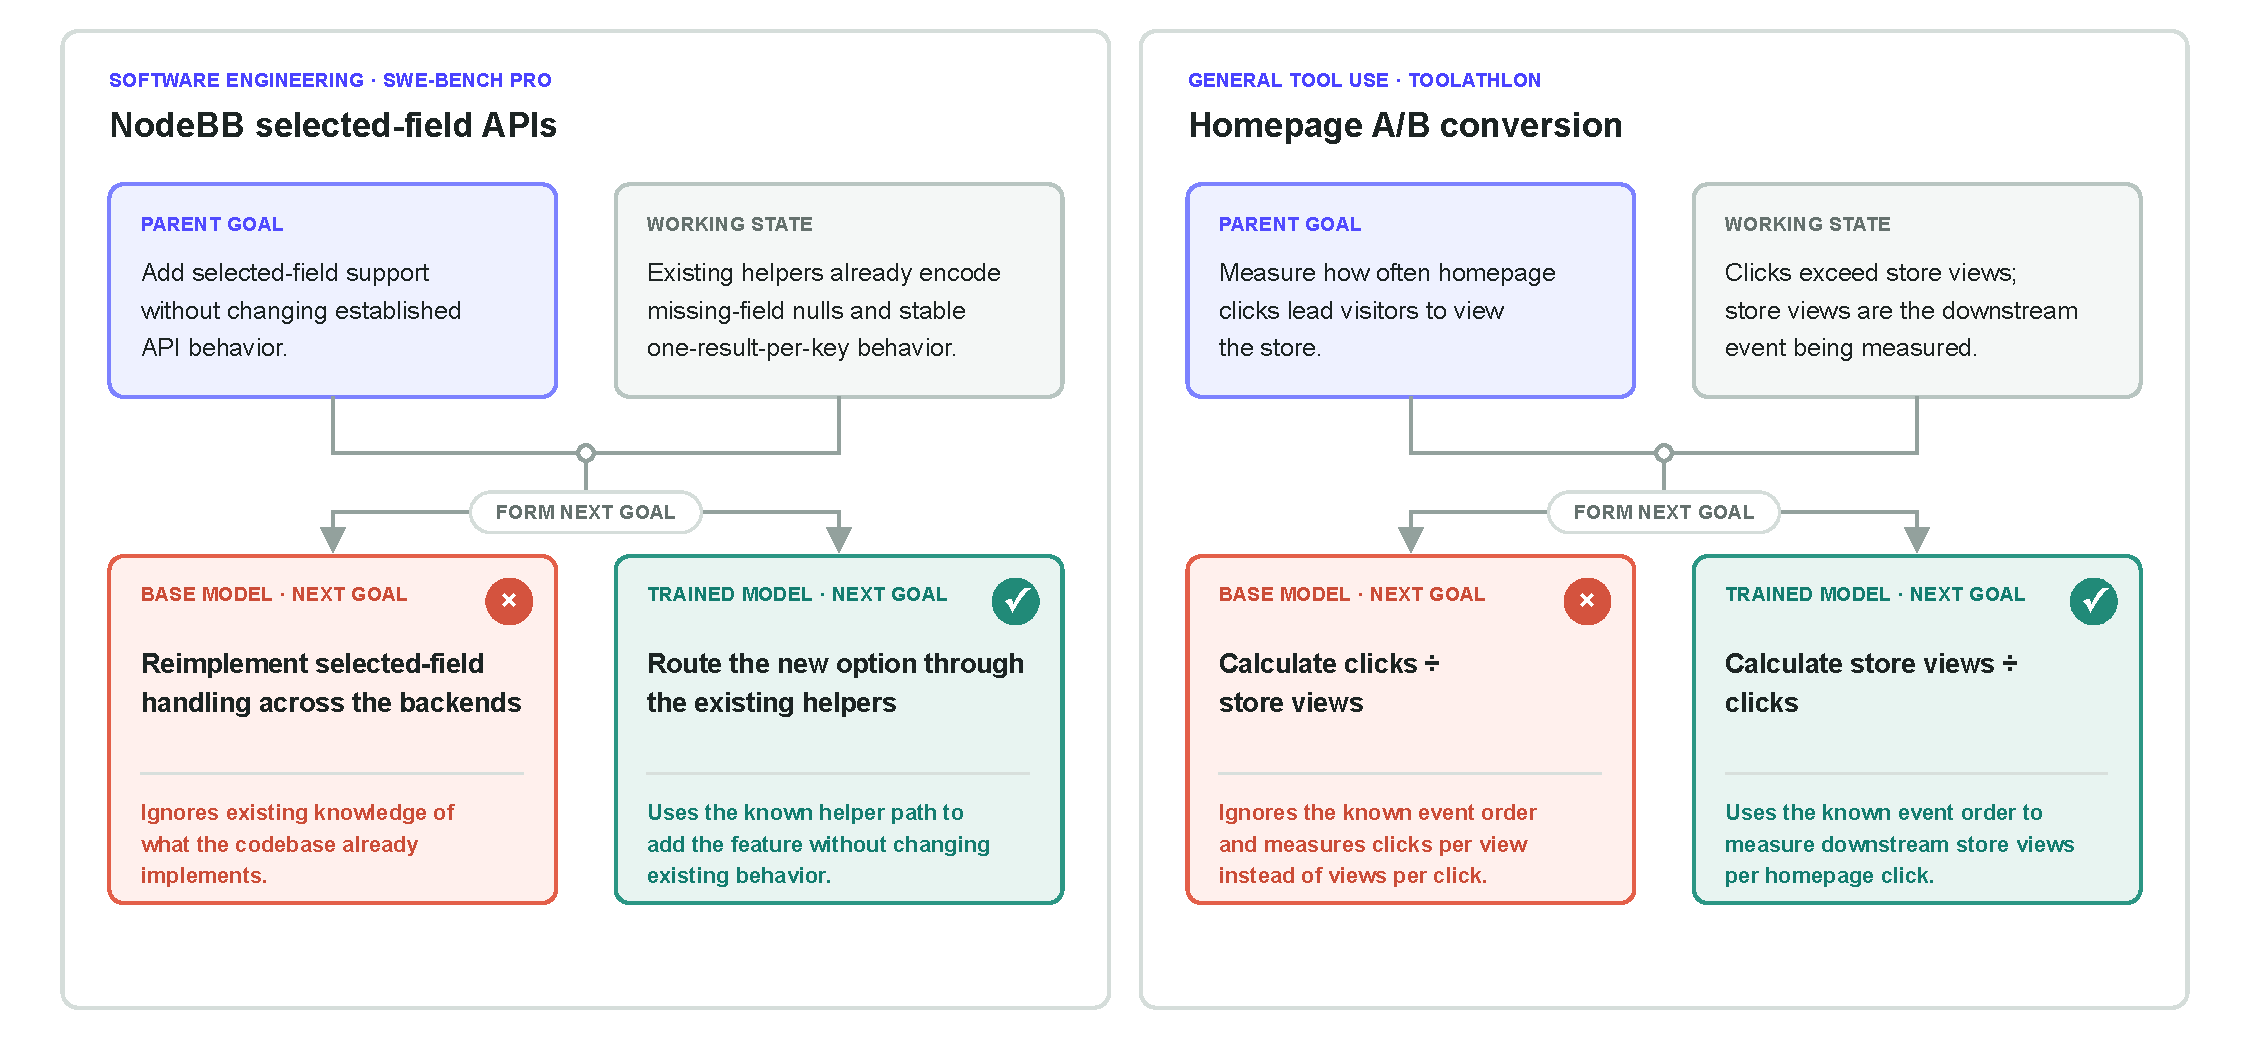
\includegraphics[width=0.9\linewidth]{figures/defining_the_right_goal.pdf}
\caption{跨领域的目标形成。面对相同的父目标和工作状态，基础模型形成了局部合理但错误的局部目标，而训练后模型形成了正确目标。}
\label{fig:goalcontrast}
\end{figure}

\paragraph{状态构建。}
智能体必须决定检查什么，并把观察整合为支持局部和更高层决策的工作状态。相关证据可能被遗漏、误解，或只在低层子任务中得到理解。

\textbf{SWE-Bench Pro：Ansible 集合名称验证。}任务要求集合名称验证器拒绝 Python 保留关键字。基础模型检查了相关导入和验证结构，随后引入了一个调用 \texttt{keyword.iskeyword} 的辅助函数，尽管该模块其实直接导入了 \texttt{iskeyword}。由此产生的 \texttt{NameError} 导致 19 项测试失败。自测暴露问题后，模型修改了测试设置，却没有改动自己的实现。训练后模型将要求与代码仓库中央的 \texttt{AnsibleCollectionRef.is\_valid\_collection\_name} 验证器联系起来，并复用了这一路径。

\textbf{Toolathlon：由公式支持的工作簿数值。}一项市场研究任务要求使用公式单元格计算同比增长。基础模型在提取时遇到公式字符串，便将相关条目作为非数值丢弃，尽管报告需要这些单元格的计算值。训练后模型使用缓存的公式结果重新打开工作簿，并保留了计算数据。两个模型遇到了相同的工具阻力，但只有训练后模型把观察整合进父目标所需的状态（图~\ref{fig:statecontrast}）。

\begin{figure}[H]
\centering
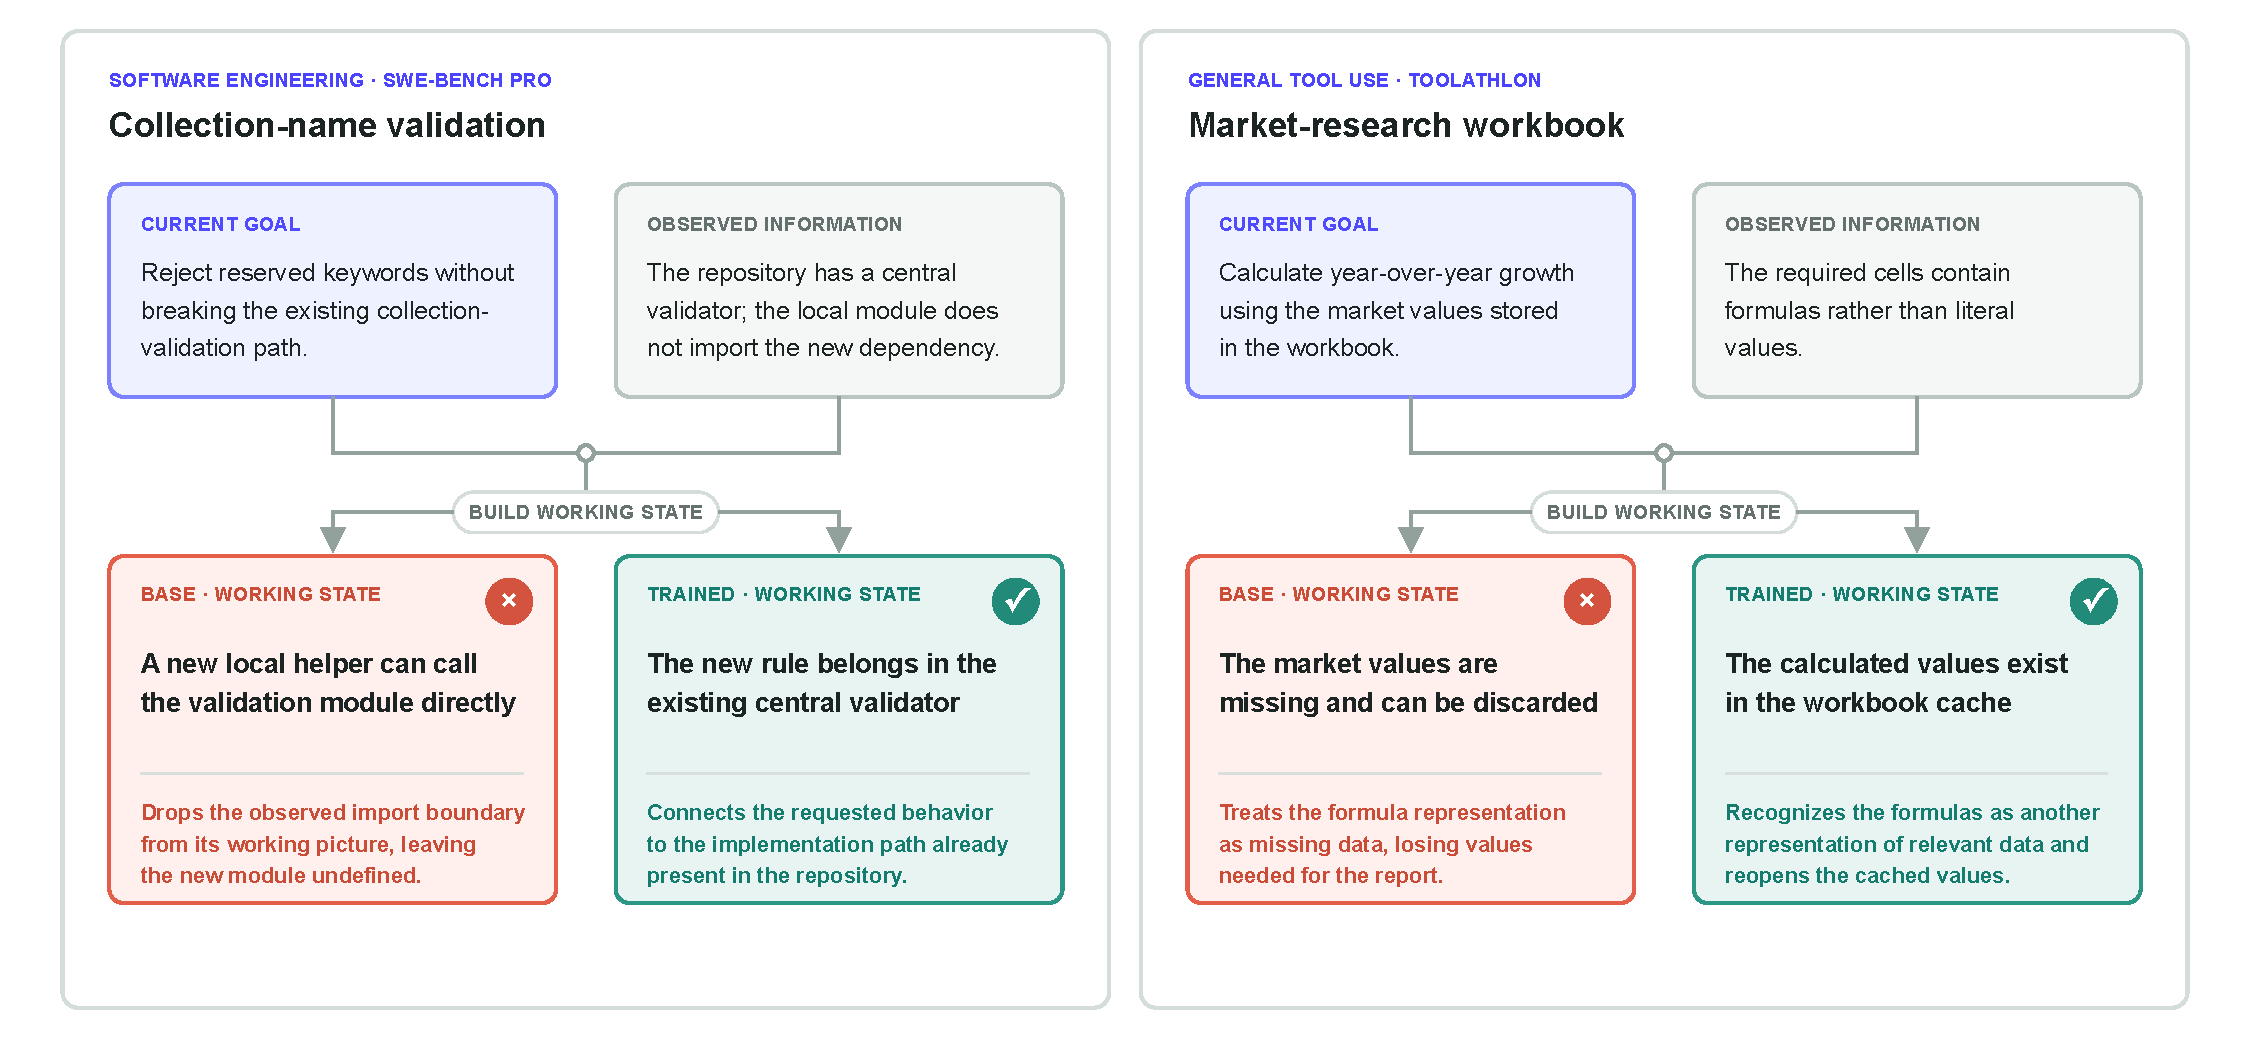
\includegraphics[width=0.9\linewidth]{figures/building_goal_relevant_state.pdf}
\caption{跨领域的状态构建。基础模型丢弃了相关观察或对其作出错误表示；训练后模型将其纳入父目标使用的工作状态。}
\label{fig:statecontrast}
\end{figure}

\paragraph{目标稳定性。}
困难的局部子任务可能取代模型先前正确表示的一项要求。

\textbf{SWE-Bench Pro：PowerShell CLIXML 解析。}解析器必须解码转义字符，同时保留回车和换行等控制字符。基础模型起初正确实现了这一要求。随后，它遇到一项现有测试，该测试预期删去末尾的 CRLF，于是模型修改实现以满足这一过时行为。训练后模型根据任务要求解释该测试，并保留了保存 CRLF 的实现。

\textbf{LHMTA 留出集：课程安排。}每门入选课程都必须属于二年级的 \texttt{2xxx} 层级。基础模型记录了这一约束，并正确识别出 \texttt{STAT1010} 无效。后来，在修复某学期负担过重的问题时，它却选择 \texttt{STAT1010} 作为选修课，并声称所有课程都符合规则。训练后模型维持了约束，选择 \texttt{ENG2010}，并移动另一门课程来解决负担过重问题。在两对轨迹中，局部修复压力都让基础模型丢失了已知的父目标标准，而训练后模型没有如此（图~\ref{fig:stabilitycontrast}）。

\begin{figure}[H]
\centering
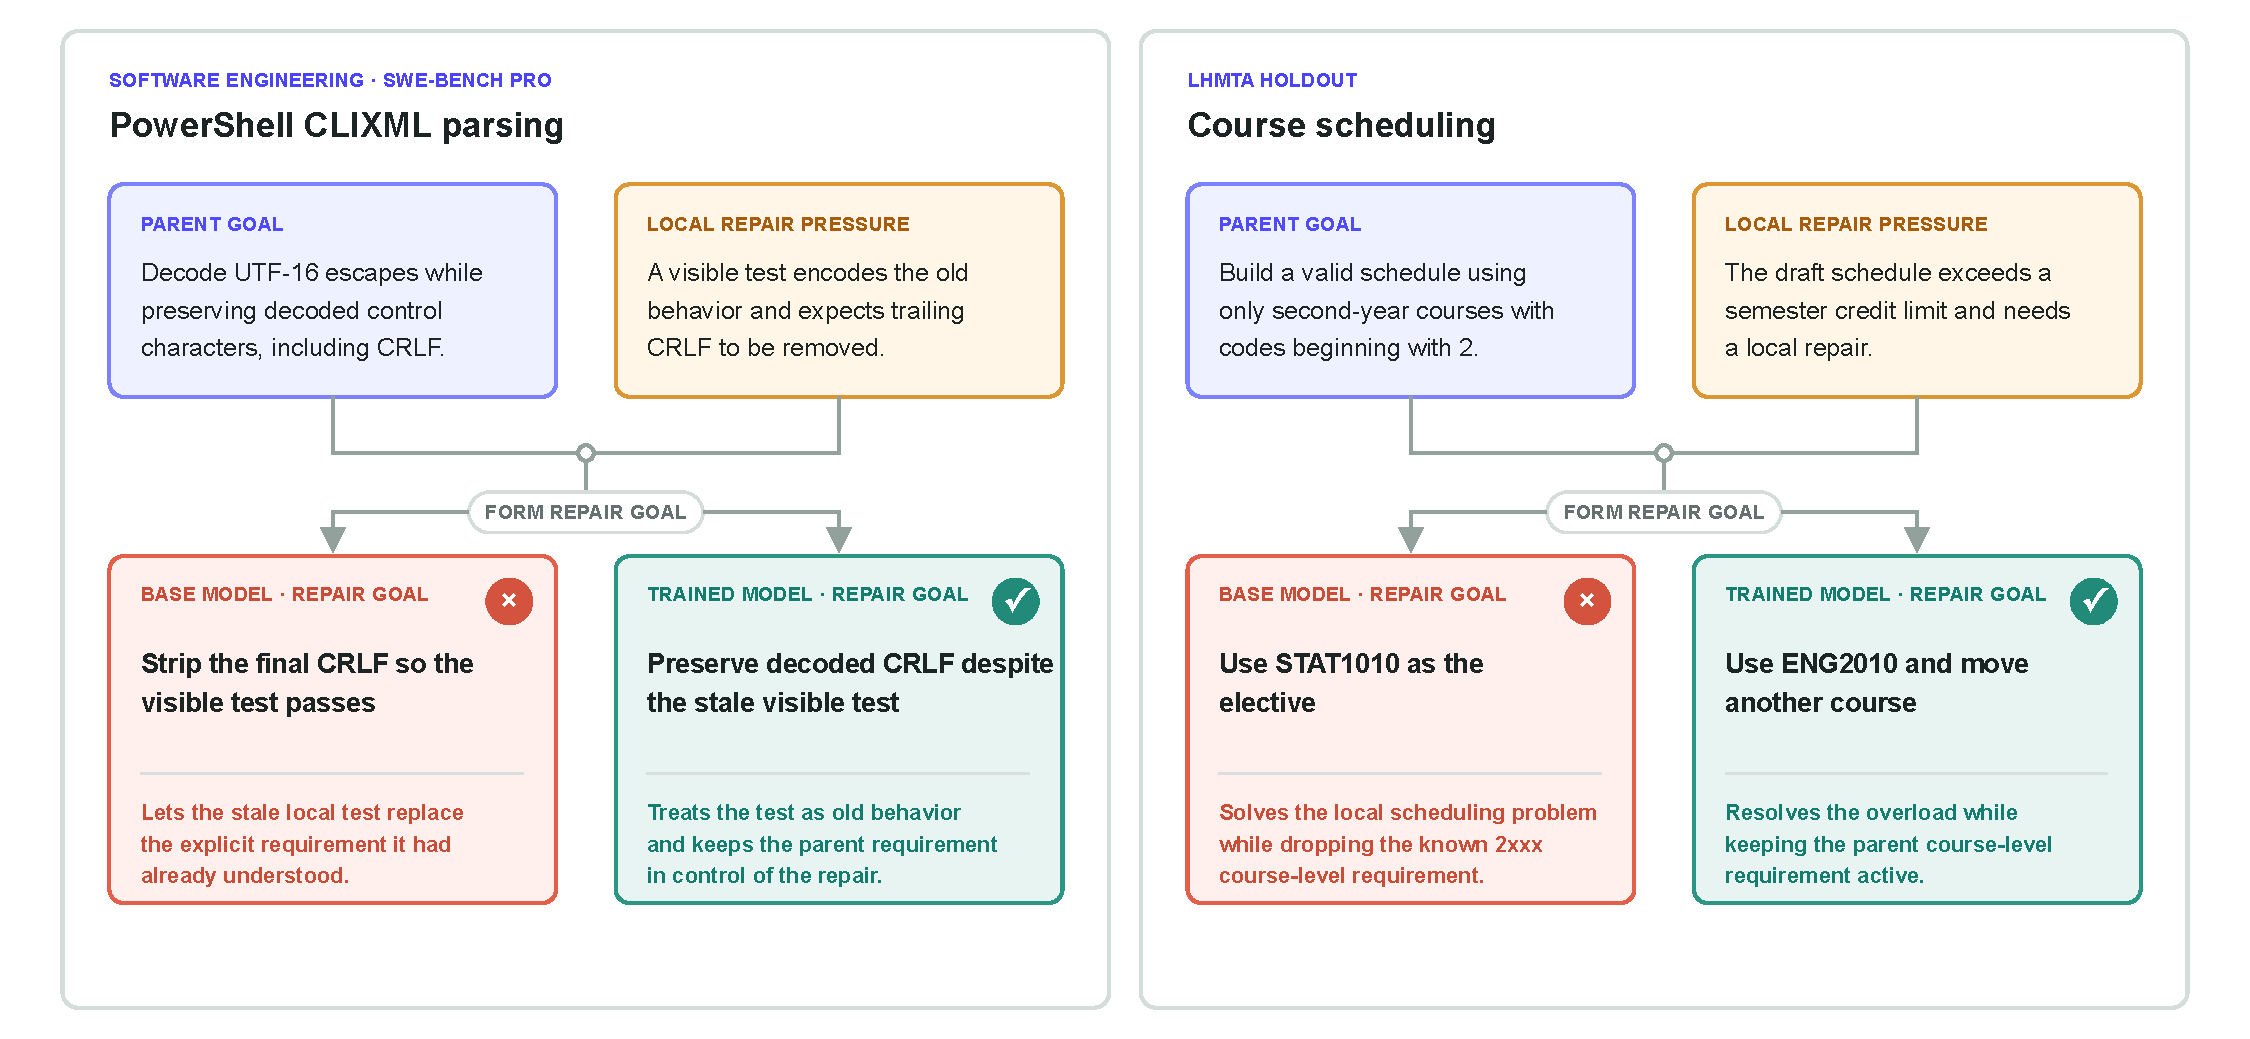
\includegraphics[width=0.9\linewidth]{figures/keeping_parent_goal_stable.pdf}
\caption{跨领域的目标稳定性。一个父目标约束进入局部修复循环；基础模型丢失了该约束，而训练后模型维持了它。}
\label{fig:stabilitycontrast}
\end{figure}

\paragraph{验证。}
验证会在任务和子任务边界闭合目标循环。模型必须判断，哪些证据能证明预期的环境状态已经达成。

\textbf{SWE-Bench Pro：Element Web 的 \texttt{Pill} 重构。}任务要求将 \texttt{Pill} 类组件改为函数组件，并导出原本是静态方法的辅助函数。基础模型检查了新辅助函数是否已被导出和导入。它的验证在搜索已删除静态 API 的调用方之前就停止了，因此下游代码仍调用 \texttt{Pill.roomNotifPos} 和 \texttt{Pill.roomNotifLen}。训练后模型搜索了过时用法，迁移调用点，并运行有针对性的 TypeScript 检查。

\textbf{LHMTA 留出集：目录核对。}一项图书馆任务要求依据分散在多个文件中的记录，核对历史类图书。基础模型通过一次有范围限制的电子表格读取生成了包含 44 本书的中间文件并检查该文件，却从未验证这次读取是否覆盖完整目录。训练后模型比较了工作簿的两个视图，确认每个视图都包含相同的 347 位历史类作者后，才使用提取结果。基础模型的检查只能证明工件存在且内部一致；训练后模型的检查则对照环境检验了相关主张（图~\ref{fig:verifycontrast}）。

\begin{figure}[H]
\centering
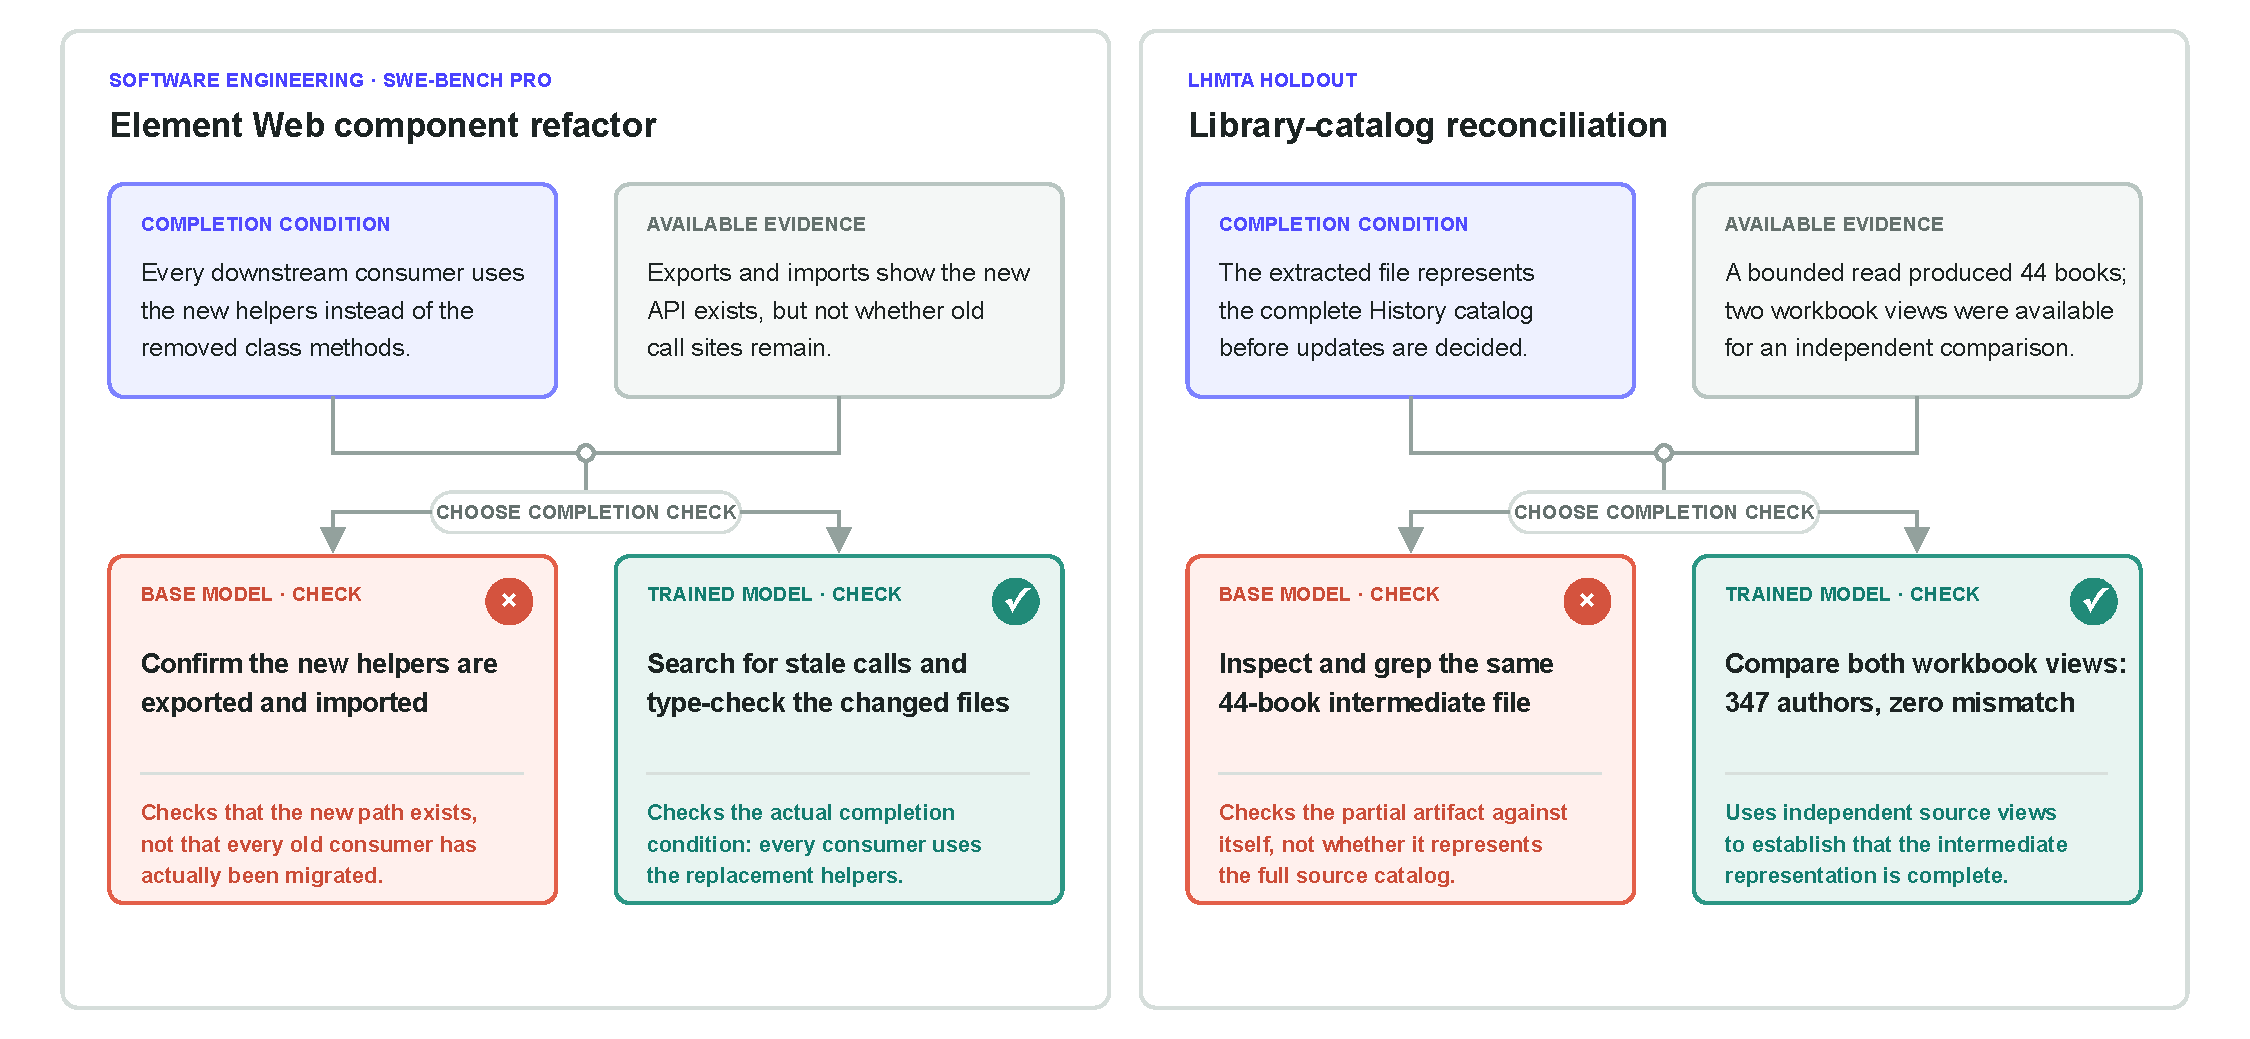
\includegraphics[width=0.9\linewidth]{figures/checking_goal_completion.pdf}
\caption{跨领域的验证。基础模型依赖代理证据或自指证据；训练后模型依据环境检验相关主张。}
\label{fig:verifycontrast}
\end{figure}

\subsection{汇总行为证据}
\label{sec:aggregate}

案例研究展示了单项任务如何产生分歧；SWE-Bench Pro 的汇总指标则考察相关行为信号是否在更广范围内出现（表~\ref{tab:metrics}）。

\begin{table}[H]
\centering
\small
\caption{基于 731 项配对任务计算的 SWE-Bench Pro 轨迹行为指标。}
\label{tab:metrics}
\begin{tabular}{p{0.38\linewidth}rrp{0.28\linewidth}}
\toprule
行为信号 & 基础模型 & 训练后 & 解释 \\
\midrule
每次运行的平均检索调用数 & 25.6 & 23.9 & 检索工作量相近 \\
平均不同检索信息量 & 7,985 & 9,019 & 获取更多独特内容 \\
重复检索信息占比 & 22.5\% & 14.3\% & 较少重复调查 \\
平均触及的参考补丁文件数 & 2.69 & 3.08 & 与参考文件重合更多 \\
平均新增行数 & 415.5 & 111.7 & 补丁更小 \\
包含正式测试的运行占比 & 37.5\% & 73.3\% & 验证更频繁 \\
首次测试的平均位置（已测试运行） & 70.8\% & 62.0\% & 更早验证 \\
通过测试后继续编辑的运行占比 & 5.9\% & 12.9\% & 中间验证更多 \\
\bottomrule
\end{tabular}
\end{table}

各指标定义如下：

\begin{itemize}
  \item \textbf{每次运行的平均检索调用数。}不会修改环境或重定向输出的只读检查命令，例如 ls、grep、cat 和只读 git 子命令。
  \item \textbf{平均不同检索信息量。}每次运行的检索调用输出中，不同 12 词元跨度的平均数量。
  \item \textbf{重复检索信息占比。}此前已在同一次运行中出现过的跨度比例。
  \item \textbf{平均触及的参考补丁文件数。}每次运行中，智能体最终补丁和任务参考补丁共同改动的平均文件数。
  \item \textbf{平均新增行数。}智能体最终补丁中的新增行数。
  \item \textbf{包含正式测试的运行占比。}至少有一条命令调用 pytest 或 \texttt{go test} 等标准测试运行器的运行占比。
  \item \textbf{首次测试的平均位置。}在已经运行测试的轨迹中，首次测试出现在全部命令流程中的相对位置，取值从零到一。
  \item \textbf{通过测试后继续编辑的运行占比。}某次测试通过后仍继续编辑文件的运行占比。
\end{itemize}

附录~\ref{app:metrics} 给出了每项指标的精确分类模式和解析规则。

训练后模型的检索调用略少，却覆盖了更多不同信息，且较少重复内容；这一模式与模型更好地维持“已经了解到什么、还有什么未知”的认识相一致。训练后模型也触及了更多参考补丁所修改的文件，而新增行数约为基础模型的四分之一，这与更有针对性的实现相一致。

测试行为提供了最清晰的汇总变化。训练后模型运行正式测试的轨迹数量接近翻倍，且更早开始测试。通过测试后继续编辑的情况也更常见，这表明验证经常为中间工作提供信息，而非只充当最终检查。

这些指标提供的是相互印证的行为信号，而不是对四项能力的直接测量。参考补丁并不能唯一指定一种有效实现策略，补丁更小也并非天然更好。现有遥测还缺乏目标稳定性的干净汇总代理指标，因此该能力的证据来自配对案例。

\section{长时程后训练教会了模型什么}
\label{sec:discussion}

结果支持一种行为学解释：后训练改变了模型组织长任务工作的方式。训练集合没有提供软件工程任务、代码仓库约定或代码级解决方案。尽管如此，目标形成、状态构建、目标稳定性和验证方面的相同差异，既出现在办公工作流中，也出现在软件代码仓库中。GDE 为这些变化提供了一种共同描述，而不要求源任务与目标任务共享主题。

一种合理解释是，训练提高了模型可靠运用预训练阶段所获知识的能力。此前研究认为，预训练模型已经包含了下游任务所需的大部分知识，而指令微调提高了模型根据用户意图运用这些知识的能力 \citep{zhou2023lima, ouyang2022instructions}。LHMTA 可能让模型在陌生而有状态的环境中追求复杂目标时，反复练习如何运用已有知识。软件工程结果具有信息价值，因为领域不匹配使模型不太可能从训练集中直接获得代码仓库特定知识。

因果解释仍然只是一项假设。实验没有分离深层分解、并行综合、相互纠缠的约束或依赖链，也没有确定这些要求中的哪一些促成了迁移。跨领域评估能够揭示训练效果何时超出表层工作流，而四项能力则为更受控的问题提供了一套词汇：哪些任务属性能强化每项能力，哪些能力会一同迁移，以及相同模式能否在不同模型、数据混合和训练方法上复现。

长时程智能体数据的编写和训练成本很高；成功的 LHMTA 轨迹往往长达 80,000 至 100,000 个词元。这使理解一次训练经历究竟锻炼了哪类行为变得更有价值。当前结果为这一问题提供了动机，但尚未给出工程化设计特定任务要求的方法。

\section{局限性}
\label{sec:limitations}

\paragraph{单一模型和单次训练。}
所有结果都来自一个基础模型和一次后训练运行。我们尚未证明这些结果能够跨随机种子、规模、模型家族、训练配方或数据混合复现。

\paragraph{探索性的行为解释。}
四项能力是在轨迹定性分析过程中反复修订得到的。它们描述目标、行动、环境证据和结果之间可观察的关系；它们既不能识别字面意义上的内部目标、状态寄存器或控制循环，也不构成完备分类体系。

\paragraph{按结果筛选的案例与分析者判断。}
分析聚焦于基础模型失败而训练后模型成功的任务，展示的案例也依据解释清晰度而非随机抽样选出。它们说明了改进如何表现出来，却无法估计每项能力的普遍程度。根据长轨迹重建目标和因果链也需要判断，而单个失败可能具有多个原因。

\paragraph{缺少因果反事实或领域匹配反事实。}
我们没有消融所提出的任务要求，也没有把 LHMTA 与等预算的软件工程训练数据进行比较。因此，实验无法证明哪些属性导致了迁移，也无法证明非软件训练是提高 SWE-Bench Pro 的最高效方式。探索、坚持性、指令遵循或工具使用等方面更广泛的变化，仍可能解释部分增益。

\paragraph{代理指标。}
检索重合度、参考文件覆盖、补丁大小和测试命令都是间接行为信号。参考补丁并非唯一的真实标准。

\section{结论}
\label{sec:conclusion}

在 363 项长时程多工具任务上对 Qwen3.5-122B-A10B 进行后训练后，模型产生了在训练领域之外仍有用的行为：尽管训练集合不含软件工程任务，SWE-Bench Pro 的性能依然提高。配对轨迹显示，目标形成、状态构建、目标稳定性和验证均反复出现改进；汇总指标则为调查、实现和测试方面的变化提供了更广泛证据。GDE 把这些差异组织成一种行为学解释，用以说明训练后模型如何推进长任务。

这些发现促使我们把后训练数据研究为锻炼行为能力的经验，而不只是包含特定主题、工具或答案的样例。确立因果关系还需要跨任务要求、领域、模型和训练方法开展受控比较。后训练科学不仅应解释一个数据集是否提高某项基准，还应解释训练经历发展了哪些行为能力，以及这些能力会迁移到哪里。

\bibliographystyle{plainnat}
\bibliography{references}

\appendix
\begin{center}
\small\emph{以下精确指标定义保留官方英文原文，以保持正则表达式与实现规则不受改写影响。}
\end{center}
\section{Exact Metric Definitions}
\label{app:metrics}

This appendix gives the exact classification rules behind the metrics in Table~\ref{tab:metrics}. All patterns are regular expressions applied case-insensitively to individual assistant shell commands. Long patterns are wrapped across lines for readability; the implemented patterns contain no whitespace at the wrap points.

\subsection{Retrieval calls}
\label{app:retrieval}

A command is classified as a retrieval call in three steps. Occurrences of \verb!>/dev/null! are ignored; any other output redirection disqualifies the command. A command matching the exclusion pattern below is disqualified. The remaining commands qualify if they match the inclusion pattern.

Inclusion pattern:

\begin{verbatim}
(?:^|[;&|()]\s*)(?:
  ls|find|fd|rg|grep|egrep|fgrep|cat|head|tail|wc|stat|file|tree|pwd|
  readlink|realpath|which|whereis|type|jq|awk|cut|sort|uniq|
  git\s+(?:show|log|grep|ls-files|rev-parse|branch|remote|blame)
)\b
\end{verbatim}

Exclusion pattern:

\begin{verbatim}
\b(?:rm|mv|cp|mkdir|rmdir|touch|chmod|chown|ln|tee|truncate|patch)\b|
\bgit\s+(?:add|commit|apply|checkout|restore|reset|clean|am|
         cherry-pick|rebase|merge)\b|
\bsed\s+-[^\n;|&]*i\b|\bperl\s+-[^\n;|&]*i\b|
\b(?:python|python3|node|ruby|php)\b|
\b(?:pytest|unittest|jest|vitest|mocha|rspec|go\s+test|cargo\s+test|
    npm\s+test|yarn\s+test|pnpm\s+test)\b|
\b(?:make|cmake|ninja|npm\s+install|yarn\s+install|pnpm\s+install|
    pip\s+install)\b|
<<
\end{verbatim}

Although \texttt{git branch} and \texttt{git remote} can mutate repository state with other arguments, all matched uses in this corpus were read-only: \texttt{git branch} appeared only in listing or inspection forms such as \verb!-a!, \verb!--contains!, and \verb!--show-current!, and \texttt{git remote} appeared only as \verb!git remote -v!. No branch creation, branch deletion, or remote mutation was counted as retrieval.

\subsection{Information spans}
\label{app:spans}

Retrieval-call outputs are processed as follows: ANSI escape sequences are removed, the text is tokenized with the pattern \verb![A-Za-z_][A-Za-z0-9_]*|\d+(?:\.\d+)?|[^\s]! and lowercased, and every overlapping window of 12 consecutive tokens forms one span; an output shorter than 12 tokens forms a single span. Distinct retrieved information is the number of unique spans in a run. Repeated retrieved information is the share of spans that already occurred in an earlier output of the same run.

\subsection{Formal tests and mutations}
\label{app:tests}

A command contains a formal test if it matches any of:

\begin{verbatim}
(?:^|[;&|]\s*|\s)(?:python\d*\s+-m\s+)?pytest(?:\s|$)
(?:^|[;&|]\s*|\s)py\.test(?:\s|$)
\bgo\s+test\b
\bcargo\s+test\b
\b(?:npm|pnpm|yarn)\s+(?:run\s+)?test(?:\s|$|:)
\b(?:npx\s+)?(?:jest|vitest|mocha)(?:\s|$)
\bmake\s+(?:[\w.-]*test[\w.-]*|check)(?:\s|$)
(?:^|[;&|]\s*|\s)(?:tox|nosetests|unittest)(?:\s|$)
\bpython\d*\s+-m\s+unittest\b
\bbazel\s+test\b
\bgradle\w*\s+test\b
\bmvn\w*\s+(?:test|verify)\b
\bdotnet\s+test\b
\brspec(?:\s|$)
\end{verbatim}

A test counts as passing when it returns code zero, is not part of a status-masking pipeline or fallback, and its output contains no explicit failure marker. A command counts as a mutation if it matches any of:

\begin{verbatim}
\bapply_patch\b
\b(?:sed|perl)\b[^\n]*(?:\s-i\b|--in-place)
\bgit\s+(?:apply|checkout|restore|reset|cherry-pick)\b
\b(?:cp|mv|rm|touch)\s+(?![^\n]*(?:/tmp/|/dev/))
\.(?:write_text|write_bytes)\s*\(
\bopen\s*\([^\n]{0,180},\s*['"](?:w|a|x|w\+|a\+)['"]
\b(?:cat|printf|echo)\b[^\n]*(?:>>|>)\s+(?!/tmp/|/dev/)[^\s;&|]+
\btee\s+(?:-a\s+)?(?!/tmp/|/dev/)[^\s;&|]+
\end{verbatim}

First-test position is the ordinal position of the first formal-test command among all of a run's assistant shell commands, normalized to the range zero to one.

\subsection{Patch metrics}
\label{app:patches}

The agent patch is the final submitted diff for a run. The reference patch is the task's gold code patch; the task's separate test patch is not included. File paths are read from \verb!diff --git! headers. Reference-patch files touched is the number of distinct files appearing in both the agent patch and the reference patch. Added lines is the number of lines beginning with \verb!+!, excluding \verb!+++! file headers, summed over all files in the agent patch.


\end{document}
